%----------------------------------------------------------------------------------------
%	PACKAGES AND OTHER DOCUMENT CONFIGURATIONS
%----------------------------------------------------------------------------------------

\documentclass[11pt, a4paper, oneside]{Thesis} % Paper size, default font size and one-sided paper

\graphicspath{{./figures/}} % Specifies the directory where pictures are stored

\usepackage[square, numbers, comma, sort&compress]{natbib} % Use the natbib reference package - read up on this to edit the reference style; if you want text (e.g. Smith et al., 2012) for the in-text references (instead of numbers), remove 'numbers' 
\hypersetup{urlcolor=black, colorlinks=true} % Colors hyperlinks in blue - change to black if annoying
\title{\ttitle} % Defines the thesis title - don't touch this

\usepackage{tikz}
\usepackage{setspace}

\definecolor{OrangeGSSI}{RGB}{237,113,45}
\definecolor{blue}{RGB}{25,25,112}

%----------------------------------------------------------------------------------------
%	DOCUMENT VARIABLES
%	Fill in the lines below to update the thesis template
%	If you wish to cite each of the variables defined below, look at the
%	section above for the citation command e.g. \examiner{} below is
%	defined as \examname above so you cite it as \examname
%----------------------------------------------------------------------------------------

\thesistitle{Topological and Numerical Stability of Higher-Order Laplacian Operators on Simplicial Complexes} % Your thesis title - this is used in the title and abstract
%-------------------------------------------------  
\supervisor{Prof.~Francesco~\textsc{Tudisco} and Prof.~Nicola~\textsc{Guglielmi}} % You supervisor's name - this is used in the title page
%-------------------------------------------------   
\examiner{Dr. Name  \textsc{Surname}} % Your examiner's name - this is not currently used anywhere in the template, cite it with \examname if you want it
%-------------------------------------------------   
\degree{Doctor of Philosophy} % Your degree name - this is currently used in the title page and abstract
%-------------------------------------------------   
\authors{Anton \textsc{Savostianov}} % Your name - this is used in the title page and abstract
%-------------------------------------------------

%----------------------------------------------------------------------------------------
%	TYPESETTING
%----------------------------------------------------------------------------------------
\usepackage{pifont}
\usepackage{xcolor,colortbl}
\usepackage{flushend}
\usepackage[normalem]{ulem} % for \sout
\usepackage{multicol}
\usepackage{xcolor}
\newcommand{\ugh}[1]{\textcolor{red}{\uwave{#1}}} % please rephrase
\newcommand{\ins}[1]{\textcolor{blue}{\uline{#1}}} % please insert
\newcommand{\del}[1]{\textcolor{red}{\sout{#1}}} % please delete
\newcommand{\chg}[2]{\textcolor{red}{\sout{#1}}{\ra}\textcolor{blue}{\uline{#2}}} % please change

\renewcommand{\ttdefault}{cmr}

\newcommand{\assignedto}[1]{\textcolor{red}{\ding{46}~{\sf Assigned to:}~#1}\\}
\newcommand{\todo}[1]{\textcolor{blue}{\ding{46}{\sf}~#1}}

\newcommand{\sugg}[1]{\textcolor{orange}{#1}}
%----------------------------------------------------------------------------------------
%	End of TYPESETTING
%----------------------------------------------------------------------------------------


\usepackage{tikz-network}
\usepackage{faktor}


%%%% COMMANDS %%%%%%%%%%%%%%%%%%%%%%%%

\newcommand*{\insidefigure}[3][0.5\columnwidth]{
      \begin{center}
            \begin{minipage}{#1}
                  \centering
                  #2
                  \captionof{figure}{#3}
            \end{minipage}
      \end{center}
}

\newcommand*{\mc}[1]{\mathcal{#1}}
\renewcommand*{\b}[1]{\mathbf{#1}}
\newcommand*\eps{\varepsilon}
\newcommand*{\V}[1]{ \mc V_{#1}(\mc K)}
\newcommand*{\vn}{\varnothing}
\newcommand*{\ord}[1]{\mathrm{ord}\,(#1)}

\usepackage{dsfont}
\newcommand*{\ds}[1]{\mathds{#1}}

\newcommand*{\Lu}[1]{L_{#1}^{\uparrow}}
\newcommand*{\Ld}[1]{L_{#1}^{\downarrow}}

\newcommand*{\wh}[1]{\widehat{#1}}


\renewcommand*{\bar}[1]{ \overline{#1} }


\newcommand{\algname}{\texttt{HeCS}}


\DeclareMathOperator{\im}{im}
\let\span\relax
\DeclareMathOperator{\span}{span}
\DeclareMathOperator{\Sym}{Sym}









\usetikzlibrary{patterns}
\definecolor{bananamania}{rgb}{0.98, 0.91, 0.71}
\definecolor{lavender}{rgb}{0.4470588235294118, 0.5294117647058824, 0.992156862745098}
\definecolor{burntsienna}{rgb}{0.91, 0.45, 0.32}
\definecolor{airforceblue}{rgb}{0.36, 0.54, 0.66}
\definecolor{liberty}{HTML}{5158BB}
\definecolor{junglegreen}{rgb}{0.16, 0.67, 0.53}


\begin{document}

\frontmatter % Use roman page numbering style (i, ii, iii, iv...) for the pre-content pages

\setstretch{1.3} % Line spacing of 1.3

% Define the page headers using the FancyHdr package and set up for one-sided printing
\fancyhead{} % Clears all page headers and footers
\rhead{\thepage} % Sets the right side header to show the page number
\lhead{} % Clears the left side page header

% \pagestyle{fancy} % Finally, use the "fancy" page style to implement the FancyHdr headers
\newcommand{\HRule}{\rule{\linewidth}{0.5mm}} % New command to make the lines in the title page

% PDF meta-data
\hypersetup{pdftitle={\ttitle}}
\hypersetup{pdfsubject=\subjectname}
\hypersetup{pdfauthor=\authornames}
\hypersetup{pdfkeywords=\keywordnames}

%----------------------------------------------------------------------------------------
%	TITLE PAGE
%----------------------------------------------------------------------------------------

\begin{titlepage}
\begin{center}


\includegraphics[width=0.4\textwidth]{./figures/logo_GSSI}~\\[1cm]
\textsc{\Large Doctoral Thesis}\\[0.5cm] % Thesis type

\HRule \\[0.1cm] % Horizontal line
{\LARGE \bfseries Topological Stability and Preconditioning  
\\[0.3cm] of Higher-Order Laplacian Operators 
\\[0.3cm]
on Simplicial Complexes }\\[0.3cm] % Thesis title
\HRule \\[0.9cm] % Horizontal line

{\Large \textsc{PhD Program in Mathematics: XXXV cycle}}\\[2cm]

\begin{minipage}{0.4\textwidth}
\begin{flushleft} \large
\emph{Author:}\\
\bigskip \authornames \\
\href{mailto:anton.savostianov@gssi.it}{anton.savostianov@gssi.it}
%\href{http://www.johnsmith.com}{\authornames} % Author name - remove the \href bracket to remove the link
\end{flushleft}
\end{minipage}
\begin{minipage}{0.5\textwidth}
\begin{flushright} \large
\emph{Supervisor:} \\
%\href{http://www.jamessmith.com}{\supname} % Supervisor name - remove the \href bracket to remove the link  
\bigskip \supname \\
\href{mailto:francesco.tudisco@gssi.it}{francesco.tudisco@gssi.it \& nicola.guglielmi@gssi.it} \\
\bigskip \bigskip
%\emph{Internal advisor:} \\
%\bigskip \examname \\
%\href{mailto:name.surname@gssi.infn.it}{name.surname@gssi.infn.it}
\end{flushright}
\end{minipage}\\[2.2cm]
 
%\large \textit{A thesis submitted in fulfilment of the requirements\\ for the degree of \degreename}\\[0.3cm] % University requirement text
%\textit{in the}\\[0.4cm]
%\groupname\\\deptname\\[2cm] % Research group name and department name


{\large \today}\\[2.2cm] % Date

\univname \\
\addressnames
%\includegraphics{Logo} % University/department logo - uncomment to place it
 
\vfill
\end{center}

\end{titlepage}

%----------------------------------------------------------------------------------------
%	DECLARATION PAGE
%	Your institution may give you a different text to place here
%----------------------------------------------------------------------------------------

%\Declaration{
%
%\addtocontents{toc}{\vspace{1em}} % Add a gap in the Contents, for aesthetics
%
%I, \authornames, declare that this thesis titled, '\ttitle' and the work presented in it are my own. I confirm that:
%
%\begin{itemize} 
%\item[\tiny{$\blacksquare$}] This work was done wholly or mainly while in candidature for a research degree at this University.
%\item[\tiny{$\blacksquare$}] Where any part of this thesis has previously been submitted for a degree or any other qualification at this University or any other institution, this has been clearly stated.
%\item[\tiny{$\blacksquare$}] Where I have consulted the published work of others, this is always clearly attributed.
%\item[\tiny{$\blacksquare$}] Where I have quoted from the work of others, the source is always given. With the exception of such quotations, this thesis is entirely my own work.
%\item[\tiny{$\blacksquare$}] I have acknowledged all main sources of help.
%\item[\tiny{$\blacksquare$}] Where the thesis is based on work done by myself jointly with others, I have made clear exactly what was done by others and what I have contributed myself.\\
%\end{itemize}
% 
%Signed:\\
%\rule[1em]{25em}{0.5pt} % This prints a line for the signature
% 
%Date:\\
%\rule[1em]{25em}{0.5pt} % This prints a line to write the date
%}
%
%\clearpage % Start a new page

%----------------------------------------------------------------------------------------
%	QUOTATION PAGE
%----------------------------------------------------------------------------------------

%\pagestyle{empty} % No headers or footers for the following pages
%
%\null\vfill % Add some space to move the quote down the page a bit
%
%\textit{``Thanks to my solid academic training, today I can write hundreds of words on virtually any topic without possessing a shred of information, which is how I got a good job in journalism."}
%
%\begin{flushright}
%Dave Barry
%\end{flushright}
%
%\vfill\vfill\vfill\vfill\vfill\vfill\null % Add some space at the bottom to position the quote just right
%
%\clearpage % Start a new page

%----------------------------------------------------------------------------------------
%	ABSTRACT PAGE
%----------------------------------------------------------------------------------------

\addtotoc{Abstract} % Add the "Abstract" page entry to the Contents

\abstract % Add a gap in the Contents, for aesthetics
\todo{Insert here the abstract of the thesis proposal.}
\clearpage % Start a new page

%----------------------------------------------------------------------------------------
%	ACKNOWLEDGEMENTS
%----------------------------------------------------------------------------------------

%\setstretch{1.3} % Reset the line-spacing to 1.3 for body text (if it has changed)
%
%\acknowledgements{\addtocontents{toc}{\vspace{1em}} % Add a gap in the Contents, for aesthetics
%
%The acknowledgements and the people to thank go here, don't forget to include your project advisor\ldots
%}
%\clearpage % Start a new page

%----------------------------------------------------------------------------------------
%	LIST OF CONTENTS/FIGURES/TABLES PAGES
%----------------------------------------------------------------------------------------

\pagestyle{fancy} % The page style headers have been "empty" all this time, now use the "fancy" headers as defined before to bring them back

\lhead{\emph{Contents}} % Set the left side page header to "Contents"
\tableofcontents % Write out the Table of Contents

\lhead{\emph{List of Figures}} % Set the left side page header to "List of Figures"
\listoffigures % Write out the List of Figures

%\lhead{\emph{List of Tables}} % Set the left side page header to "List of Tables"
%\listoftables % Write out the List of Tables

%%----------------------------------------------------------------------------------------
%%	ABBREVIATIONS
%%----------------------------------------------------------------------------------------
%\clearpage % Start a new page
%\setstretch{1.5} % Set the line spacing to 1.5, this makes the following tables easier to read
%\lhead{\emph{Abbreviations}} % Set the left side page header to "Abbreviations"
%\listofsymbols{ll} % Include a list of Abbreviations (a table of two columns)
%{
%\textbf{AMI} & \textbf{A}dvanced \textbf{M}etering \textbf{I}nfrastructure \\
%\textbf{CPS} & \textbf{C}yber-\textbf{P}hysical \textbf{S}ystems \\
%\textbf{DoS} & \textbf{D}enial-\textbf{o}f-\textbf{S}ervice \\
%\textbf{MAC} & \textbf{M}edium \textbf{A}ccess {C}ontrol \\
%\textbf{MAPE} & \textbf{M}onitor, \textbf{A}nalyse, \textbf{P}lan, \textbf{E}xecute \\
%\textbf{MCN} & \textbf{M}ulti-hop \textbf{C}ontrol \textbf{N}etwork \\
%\textbf{MILS} & \textbf{M}ultiple \textbf{I}ndependent \textbf{L}evels of \textbf{S}ecurity/Safety\\
%\textbf{MRMC} & \textbf{M}arkov \textbf{R}eward \textbf{M}odel \textbf{C}hecker \\
%\textbf{MTD} & \textbf{M}oving \textbf{T}arget \textbf{D}efence \\
%\textbf{NICS} & \textbf{N}etworked \textbf{I}ndustrial \textbf{C}ontrol \textbf{S}ystems \\
%\textbf{OPC} & \textbf{O}bject linking and embedding for \textbf{P}rocess \textbf{C}ontrol \\
%\textbf{PCS} & \textbf{P}rocess \textbf{C}ontrol \textbf{S}ystems \\
%\textbf{PLC} & \textbf{P}rogrammable \textbf{L}ogic \textbf{C}ontroller \\
%\textbf{PRISM} & \textbf{P}robabilistic \textbf{S}ymbolic \textbf{M}odel \textbf{C}hecker \\
%\textbf{RTU} & \textbf{R}emote \textbf{T}erminal \textbf{U}nit \\
%\textbf{SCADA} & \textbf{S}upervisory \textbf{C}ontrol \textbf{A}nd \textbf{D}ata \textbf{A}cquisition\\
%\textbf{SLR} & \textbf{S}ystematic \textbf{L}iterature \textbf{R}eview \\
%\textbf{SMC} & \textbf{S}tatistical \textbf{M}odel \textbf{C}hecking \\
%\textbf{VCSE} & \textbf{V}irtual \textbf{C}ontrol \textbf{S}ystem \textbf{E}nvironment \\
%%\textbf{Acronym} & \textbf{W}hat (it) \textbf{S}tands \textbf{F}or \\
%}

%----------------------------------------------------------------------------------------
%	PHYSICAL CONSTANTS/OTHER DEFINITIONS
%----------------------------------------------------------------------------------------

%\clearpage % Start a new page
%
%\lhead{\emph{Physical Constants}} % Set the left side page header to "Physical Constants"
%
%\listofconstants{lrcl} % Include a list of Physical Constants (a four column table)
%{
%Speed of Light & $c$ & $=$ & $2.997\ 924\ 58\times10^{8}\ \mbox{ms}^{-\mbox{s}}$ (exact)\\
%% Constant Name & Symbol & = & Constant Value (with units) \\
%}

%----------------------------------------------------------------------------------------
%	SYMBOLS
%----------------------------------------------------------------------------------------

%\clearpage % Start a new page
%
%\lhead{\emph{Symbols}} % Set the left side page header to "Symbols"
%
%\listofnomenclature{lll} % Include a list of Symbols (a three column table)
%{
%$a$ & distance & m \\
%$P$ & power & W (Js$^{-1}$) \\
%% Symbol & Name & Unit \\
%
%& & \\ % Gap to separate the Roman symbols from the Greek
%
%$\omega$ & angular frequency & rads$^{-1}$ \\
%% Symbol & Name & Unit \\
%}

%----------------------------------------------------------------------------------------
%	DEDICATION
%----------------------------------------------------------------------------------------

\setstretch{1.3} % Return the line spacing back to 1.3
%
%\pagestyle{empty} % Page style needs to be empty for this page
%
%\dedicatory{For/Dedicated to/To my\ldots} % Dedication text
%
%\addtocontents{toc}{\vspace{2em}} % Add a gap in the Contents, for aesthetics

%----------------------------------------------------------------------------------------
%	THESIS CONTENT - CHAPTERS
%----------------------------------------------------------------------------------------

\mainmatter % Begin numeric (1,2,3...) page numbering

\pagestyle{fancy} % Return the page headers back to the "fancy" style

% Include the chapters of the thesis as separate files from the Chapters folder
% Uncomment the lines as you write the chapters

%\input{chapters/intro}
%\input{chapters/background} 
%\input{chapters/sota} 
%\input{chapters/proposal} 

\section{Introduction}
\section{ From Graphs to Simplicial Complex }

%\subsection{ Higher-order Models in Networks }

\subsection{ Simplicial Complexes }


Let \( V = \{ v_1, v_2, \ldots, v_n \} \) be a set of nodes; as discussed above, such set may refer to various interacting entities and agents in the system, e.g.\ neurons, genes, traffic stops, online actors, publication authors, etc. Then: 

\begin{definition}[Simplicial Complex]\label{def:simplicial_complex}
      The collection of subsets \( \mathcal K \) of the nodal set \( V \) is  a (abstract) \gls{SC}\mnl{addition of the word ``abstract'' to the term is more common in the topological setting} if for each subset \( \sigma \in \mc K \), referred as a \gls{simplex}, all its subsets \( \sigma'\), \( \sigma' \subseteq \sigma \), referred as \glspl{face}, enter \( \mc K \) as well, \( \sigma' \in \mc K\).
\end{definition}

A simplex \( \sigma \in \mc K \) on \( k + 1 \) vertices is said to be of the order \( k \), \( \ord \sigma = k \). Let \( \V k \) be a set of all \(k\)-order simplices in \( \mc K \) and \( m_k \) is the cardinality of \( \V k\), \( m_k = | \V k | \); then \( \V 0 \) is the set of nodes in the simplicial complex \( \mc K \), \( \V 1 \) --- the set of edges, \( \V 2 \) --- the set of triangles, or \(3\)-cliques, and so on, with \( \mc K = \{ \V 0, \V 1, \V 2 \ldots \} \). Note that due to the inclusion rule in \Cref{def:simplicial_complex}, the number of non-empty \( \V k \) is finite and, moreover, uninterupted in a sense of the order: if \( \V k = \vn \), then \( \V {k+1} \) is also necessarily empty.
\en{
      \insidefigure[0.3\columnwidth]{ \begin{tikzpicture}

      \fill [opacity=0.3,liberty]    (0, 0) -- (3, 0) --  (1.5, 2.6) -- cycle;
      %\node at (1.5, 0.9) {\AxisRotator[rotate=-90]};
      %\node at (1.5, 1.2) {\small \color{liberty!50!jet} +1};
      \fill [opacity=0.2,liberty]    (5.0, 1.0) -- (6.5, 2.6) --  (6.4, 1.4) -- cycle;
      %\node at (17.9/3, 5/3) {\AxisRotatorMirror[rotate=0]};
      \fill [opacity=0.6,liberty]    (5.0, 1.0) -- (9.0, -0.4) --  (6.4, 1.4) -- cycle;
      %\node at (6.8, 2/3) {\AxisRotator[rotate=-90]};
      \fill [opacity=0.4,liberty]    (6.5, 2.6) -- (9.0, -0.4) --  (6.4, 1.4) -- cycle;
      %\node at (7.3, 1.2) {\AxisRotatorMirror[rotate=-90]};
      
      


      \Vertex[x=0, y=0,style={color=persimmon}, fontcolor=white, size=0.25, label = 1]{v1}
      %\node[below left=-1pt of v1] {\small \color{persimmon}+1};
      \Vertex[x=3, y=0,style={color=persimmon}, fontcolor=white, size=0.25, label = 2]{v2}
      %\node[below=-1pt of v2] {\small \color{persimmon}-2};
      \Vertex[x=1.5, y=2.6, style={color=persimmon}, fontcolor=white, size=0.25, label = 3]{v3}
     % \node[above=-1pt of v3] {\small \color{persimmon}+0};
      \Vertex[x=5, y=1.0, style={color=persimmon}, fontcolor=white, size=0.25, label = 4]{v4}
    %  \node[above=-1pt of v4] {\small \color{persimmon}-3};
      \Vertex[x=6.5, y=2.6, style={color=persimmon}, fontcolor=white, size=0.25, label = 5]{v5}
   %   \node[above right=-1pt of v5] {\small \color{persimmon}-1};
      \Vertex[x=9, y=-.4, style={color=persimmon}, fontcolor=white, size=0.25, label = 6]{v6}
  %    \node[below=-1pt of v6] {\small \color{persimmon}+0};
      \Vertex[x=6.4, y=1.4, style={color=persimmon}, fontcolor=white, size=0.25, label = 7]{v7}
 %     \node[right=-1pt of v7] {\small \color{persimmon}+2};
      \Vertex[x=11.0, y=2.0, style={color=persimmon}, fontcolor=white, size=0.25, label = 8]{v8}
%      \node[above=-1pt of v8] {\small \color{persimmon}+3};

      \Edge[](v1)(v2)
      \Edge[](v1)(v3)
      \Edge[](v2)(v3)
      \Edge[](v2)(v4)
      \Edge[](v3)(v4)
      \Edge[](v4)(v5)
      \Edge[](v4)(v6)
      \Edge[](v4)(v7)
      \Edge[](v5)(v6)
      \Edge[](v5)(v7)
      \Edge[](v6)(v7)
      \Edge[](v6)(v8)
\end{tikzpicture} }{
            Example of a simplicial complex}}

\begin{example}[Simplicial Complex]

      123
      
\end{example}



\subsection{ Hodge's Algebra }


\chapter{Topological Stability as MNP}

\section{ General idea of the topological stability }

\subsection{Alternative with a persistent homology}


\subsection{ Transition to the spectral properties }





\section{ 101 on Spectral Matrix Nearness Problems }

\todo{definition}

Generally speaking, for a given matrix \( A \) a \emph{matrix nearness problem} consists of finding the closest possible matrix \( X \) among the admissible set with a number of desired properties. For instance, one may search for the closest (in some metric) symmetric positive/negative definite matrix, unitary matrix or the closest graph Laplacian. 

Motivated by the topological meaning of the \emph{kernel} of Hodge Laplacians \( L_k \), we assume the specific case of \emph{spectral} MNPs: here one aims for the target matrix \( X \) to have a specific spectrum \( \sigma(X) \). For instance in the stability study of the dynamical system \( \dot{\b x} = A \b x \) one can search for the closest Hurwitz matrix such that \( \mathrm{Re} \left[ \lambda_i \right] < 0 \) for all \( \lambda_i \in \sigma(X) \); similarly, assuming given matrix \( A \) is a graph Laplacian, one can search for the closest disconnected graph (so the algebraic connectivity \( \lambda_2 = 0 \)).

Here we recite the optimization framework developed by REFREFREF\todo{fix it} for the class of the spectral matrix nearness problems; one should note, however, that this is by far not the only approach to the task, REFREFREF\todo{also fix it with Nicholas and others, I guess?}.

\subsection{Functional and Gradient Flow}

Let as assume that \( X = A + \Delta \) and intead of searching for \( X \), we search for the perturbation matrix \( \Delta \); additionally, we assume that \( \Omega \) is the admissible set containing all possible perturbations \( \Delta \).


\subsection{ Transition to the gradient flow }
  
  \todo{ Derivative }

\subsection{ Constraint gradient flow }

\subsection{ Sparsity pattern and rank-1 optimizers }

\subsection{ Idea of two level optimization }















\section{Direct approach: failure and discontinuity problems }


\subsection{Principal spectral inheritance}


Before moving on to the next section, we recall here a relatively direct  but important spectral property that connects the spectra of the $k$-th and $(k+1)$-th order Laplacians. 

\begin{theorem}[HOL's spectral inheritance]\label{thm:inherit}
  Let $L_k$ and $L_{k+1}$ be  higher-order Laplacians for the same simplicial complex $\mc K$. Let $\bar L_k=\bar L_k^{down}+\bar L_k^{up}$, where $\bar L_k^{down}=\bar B_k^\top \bar B_k$ and $\bar L_k^{up}=\bar B_{k+1} \bar B_{k+1}^\top$. Then:
  \begin{enumerate}
    \item $\sigma_+(\bar L_k^{up})=\sigma_+(\bar L_{k+1}^{down})$, where $\sigma_+(\cdot)$ denotes the positive part of the spectrum;
    \item if $ 0 \ne \mu \in \sigma_+(\bar L_k^{up}) = \sigma_+(\bar L_{k+1}^{down})$, then the eigenvectors are related as follows:
    \begin{enumerate}
      \item if $\b x$ is and eigenvector for $\bar L_k^{up}$ with the eigenvalue $\mu$, then $\b y = \frac{1}{\sqrt{\mu}} \bar B_{k+1}^\top \b x$ is an eigenvector for $\bar L_{k+1}^{down}$ with the same eigenvalue;
      \item if $\b u$ is and eigenvector for $\bar L_{k+1}^{down}$ with the eigenvalue $\mu$ and $\b u \notin \ker \bar B_{k+1}$, then $\b v = \frac{1}{\sqrt{\mu}} \bar B_{k+1} \b u$ is an eigenvector for $\bar L_{k}^{up}$ with the same eigenvalue;
    \end{enumerate}
    \item for each Laplacian $\bar L_k$: if $\b v \notin \ker \bar L_k^{down}$ is the eigenvector for $\bar L_k^{down}$, then $\b v \in \ker \bar L_{k}^{up}$; vice versa, if $\b u \notin \ker \bar L_k^{up}$ is the eigenvector for $\bar L_k^{up}$, then $\b v \in \ker \bar L_k^{down}$;
    \item consequently, there exist $\mu \in \sigma_+(\bar L_k)$ with an eigenvector $\b u \in \ker \bar L_k^{up}$, and $\nu \in \sigma_+(\bar L_{k+1})$ with an eigenvector $\b u \in \ker \bar L_{k+1}^{down}$, such that:
    $$
    \bar B_k^\top \bar B_k \b v  = \mu \b v, \qquad \bar B_{k+2} \bar B_{k+2}^\top \b u = \nu \b u\, . 
    $$
  \end{enumerate}
\end{theorem}
\begin{proof}
For $(2a)$ it is sufficient to note that $ \bar L_{k+1}^{down} \b y = \bar B_{k+1}^\top \bar B_{k+1} \frac{1}{\sqrt{\mu}} \bar B_{k+1}^\top \b x = \frac{1}{\sqrt{\mu}}\bar B_{k+1}^\top \bar L_k^{up} \b x = \sqrt \mu \bar B_{k+1}^\top \b x  = \mu \b y$. Similarly, for $(2b)$: $\bar L_k^{up} \b v= \bar B_{k+1} \bar B_{k+1}^\top \frac{1}{\sqrt{\mu}} \bar B_{k+1} \b u = \frac{1}{\sqrt{\mu}} \bar B_{k+1} \bar L_{k+1}^{down} \b u = \mu \b v $; joint $2(a)$ and $2(b)$ yield $(1)$. \emph{Hodge decomposition} immediately yields the strict separation of eigenvectors between $\bar L_k^{up}$ and $\bar L_k^{down}$, $(3)$; given $(3)$, all the inherited  eigenvectors from $(2a)$ fall into the $\ker \bar L_{k+1}^{down}$, thus resulting into $(4)$.
\end{proof}
In other words, the variation of the spectrum of the $k$-th Laplacian when moving from one order to the next one works as follows: 
the down-term $\bar L_{k+1}^{down}$ inherits the positive part of the spectrum from the up-term of  $\bar L_k^{up}$; the  eigenvectors corresponding to the inherited positive part of the spectrum lie in the kernel of $\bar L_{k+1}^{up}$; at the same time, the ``new'' up-term $\bar L_{k+1}^{up}$ has a new, non-inherited, part of the positive spectrum (which, in turn, lies in the kernel of the $(k+2)$-th down-term).

In particular, we notice that for $k = 0$, since $B_0=0$ and $\bar L_0=\bar L_0^{up}$, the  theorem yields $\sigma_+ (\bar L_0 ) = \sigma_+ (\bar{L_1}^{down}) \subseteq \sigma_+(\bar L_1)$. In other terms, the positive spectrum of the $\bar L_0$ is inherited by the spectrum of $\bar L_1$ and the remaining (non-inherited) part of $\sigma_+(\bar L_1)$ coincides with $\sigma_+(\bar L_1^{up})$. 
\Cref{fig:thm_spct_ill} provides an  illustration of the statement of  \Cref{thm:inherit} for $k = 0$.
  \begin{figure}[t]
    \centering
    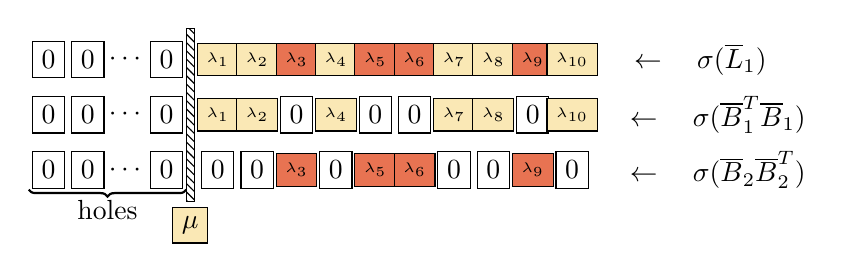
\begin{tikzpicture}
      \node[draw] at (0,0) {0};
      \node[draw] at (0.5,0) {0};
      \node at (1, 0) {$\cdots$};
      \node[draw] at (1.5,0) {0};
      \node[draw, fill=bananamania] at (2.15,0) {\tiny{$\lambda_1$}};
      \node[draw, fill=bananamania] at (2.65,0) {\tiny{$\lambda_2$}};
      \node[draw, fill=burntsienna] at (3.15,0) {\tiny{$\lambda_3$}};
      \node[draw, fill=bananamania] at (3.65,0) {\tiny{$\lambda_4$}};
      \node[draw, fill=burntsienna] at (4.15,0) {\tiny{$\lambda_5$}};
      \node[draw, fill=burntsienna] at (4.65,0) {\tiny{$\lambda_6$}};
      \node[draw, fill=bananamania] at (5.15,0) {\tiny{$\lambda_7$}};
      \node[draw, fill=bananamania] at (5.65,0) {\tiny{$\lambda_8$}};
      \node[draw, fill=burntsienna] at (6.15,0) {\tiny{$\lambda_9$}};
      \node[draw, fill=bananamania] at (6.65,0) {\tiny{$\lambda_{10}$}};
      \node at (8.5, 0) {$\leftarrow \quad \sigma (\bar L_1)$\phantom{$\bar B_1$}};
    
      \node[draw] at (0,-0.7) {0};
      \node[draw] at (0.5,-0.7) {0};
      \node at (1, -0.7) {$\cdots$};
      \node[draw] at (1.5,-0.7) {0};
      \node[draw, fill=bananamania] at (2.15,-0.7) {\tiny{$\lambda_1$}};
      \node[draw, fill=bananamania] at (2.65,-0.7) {\tiny{$\lambda_2$}};
      \node[draw] at (3.15,-0.7) {0};
      \node[draw, fill=bananamania] at (3.65,-0.7) {\tiny{$\lambda_4$}};
      \node[draw] at (4.15,-0.7) {0};
      \node[draw] at (4.65,-0.7) {0};
      \node[draw, fill=bananamania] at (5.15,-0.7) {\tiny{$\lambda_7$}};
      \node[draw, fill=bananamania] at (5.65,-0.7) {\tiny{$\lambda_8$}};
      \node[draw] at (6.15,-0.7) {0};
      \node[draw, fill=bananamania] at (6.65,-0.7) {\tiny{$\lambda_{10}$}};
      \node at (8.5, -0.7) {$\leftarrow \quad \sigma (\bar B_1^T \bar B_1)$};
    
      \node[draw] at (0,-1.4) {0};
      \node[draw] at (0.5,-1.4) {0};
      \node at (1, -1.4) {$\cdots$};
      \node[draw] at (1.5,-1.4) {0};
      \node[draw] at (2.15,-1.4) {0};
      \node[draw] at (2.65,-1.4) {0};
      \node[draw, fill=burntsienna] at (3.15,-1.4) {\tiny{$\lambda_3$}};
      \node[draw] at (3.65,-1.4) {0};
      \node[draw, fill=burntsienna] at (4.15,-1.4) {\tiny{$\lambda_5$}};
      \node[draw, fill=burntsienna] at (4.65,-1.4) {\tiny{$\lambda_6$}};
      \node[draw] at (5.15,-1.4) {0};
      \node[draw] at (5.65,-1.4) {0};
      \node[draw, fill=burntsienna] at (6.15,-1.4) {\tiny{$\lambda_9$}};
      \node[draw] at (6.65,-1.4) {0};
      \node at (8.5, -1.4) {$\leftarrow \quad \sigma (\bar B_2 \bar B_2^T)$};
    
      \draw [
        thick,
        decoration={
            brace,
            mirror,
            raise=0.25cm
        },
        decorate
      ] (-0.25, -1.4) -- (1.75, -1.4) 
    node [pos=0.5,anchor=north,yshift=-0.25cm] {holes}; 
      \draw[pattern=north west lines] (1.75,0.4) rectangle (1.85, -1.8);
      \node[draw, align=center, fill=bananamania] at (1.8,-2.1) {$\mu$};
    \end{tikzpicture}
    \caption{Illustration for the principal spectrum inheritance (\Cref{thm:inherit}) in case $k=0$: spectra of $\bar L_1$, $\bar {\Ld 1}$ and $\bar {\Ld 1}$ are shown. Colors signify the splitting of the spectrum, $\lambda_i>0 \in \sigma(\bar L_1)$ ; all yellow eigenvalues are inherited from $\sigma_+(\bar L_0)$; red eigenvalues belong to the non-inherited part. Dashed barrier $\mu$ signifies the penalization threshold (see the target functional in \Cref{subsec:functional}) preventing homological pollution (see \Cref{subsec:connetedness}). }
    \label{fig:thm_spct_ill}
    \vspace{-10pt}
  \end{figure}


\subsection{ Example with inheritted disconnectedness }



\subsection{ Example with faux edges (different weighting scheme) }





\section{ Functional, derivative and alternating scheme }

\subsection{ Target Functional }


\subsection{ Free gradient calculation }

\begin{theorem}[Derivative of simple eigenvalues]\label{lem:eigderiv} 
  Consider a continuously differentiable path of square symmetric matrices $A(t)$ for $t$ in an open interval $\mc I$. Let $\lambda(t)$, $t\in \mc I$, be a continuous path of simple eigenvalues of $A(t)$. Let $\vec x(t)$ be the eigenvector associated to the eigenvalue $\lambda(t)$ and assume
  $\| \vec x(t) \| = 1$ for all $t$. 
  Then $\lambda$ is continuously differentiable on $\mc I$ with the derivative (denoted by a dot) 
  \begin{equation}
  \dot{\lambda} = \vec x^\top \dot{A} \vec x = \langle \vec  x \vec x^\top, \dot A \rangle\,.
  \end{equation}
  Moreover, ``continuously differentiable'' can be replaced with ``analytic'' in the assumption and the conclusion.
  \end{theorem}
  
  Let us denote the perturbed weight matrix by $\tilde W_1 (t) = W_1 + \eps E(t)$, and the corresponding $\tilde W_0 (t) = W_0(\tilde W_1(t))$ and $ \tilde W_2 (t) = W_2 (\tilde W_1(t) )$, defined accordingly as discussed in Section~\ref{sec:nearest_complex}. From now on
  we omit the time dependence for the perturbed matrices to simplify the notation.  
  Since $\tilde W_0$, $\tilde W_1$ and $\tilde W_2$ are necessarily diagonal, by the chain rule we have $\dot{\tilde{W}}_i (t) = \eps \diag \left( J_1^i  \dot E \vec 1  \right)$, where $\vec 1$ is the vector of all ones, $\diag(\vec v)$ is the diagonal matrix with diagonal entries the vector $\vec v$, and  $J_1^i$ is the Jacobian matrix of the $i$-th weight matrix with respect to $\tilde W_1$, which for any $u_1\in \mathcal V_1$ and $u_2 \in \mathcal V_i$, has entries 
  \(
      [J_1^i]_{u_1,u_2}=\frac{\partial }{\partial \tilde{w}_1{(u_1)}}\tilde{w}_i{(u_2)}\, .
  \)
  
  Next, in the following two lemmas, we express the time derivative of the Laplacian $\bar L_0$ and $\bar L_1^{up}$ as functions of $E(t)$. The proofs of these results are  straightforward and omitted for brevity. In what follows, $\Sym[A]$ denotes the symmetric part of the matrix $A$, namely $\Sym[A] = (A+A^\top)/2$.
  
  
  \begin{lemma}[Derivative of $\bar L_0$]
    \label{lem:eigderL0} 
    For the simplicial complex $\mc K$ with the initial edges' weight matrix $W_1$ and  fixed perturbation norm $\eps$, let $E(t)$ be a smooth path and $\tilde W_0, \tilde W_1, \tilde W_2$ be corresponding perturbed weight matrices. Then,
    \begin{equation}
      \frac{1}{2\eps} \frac{d}{dt} \bar L_0 (t)  = \tilde W_0^{-1}  B_1 \tilde W_1 \dot E  B_1^\top \tilde W_0^{-1}-\Sym\left[ \tilde W_0^{-1} \diag \left(  J_1^0 \dot E \vec 1 \right)  \bar L_0 \right]. 
    \end{equation}
  \end{lemma}
  
  \begin{lemma}[Derivative of $\bar L_1^{up}$]
    \label{lem:eigderL1}
    For the simplicial complex $\mc K$ with the initial edges' weight matrix $W_1$ and fixed perturbation norm $\eps$,  let $E(t)$ be a smooth path and $\tilde W_0, \tilde W_1, \tilde W_2$ be corresponding perturbed weight matrices.  Then, 
    \begin{equation*}
     \frac{1}{2\eps} \frac{d}{dt} \bar L^{up}_1 (t)  =   - \Sym \left[ \tilde W_1^{-1} B_2 \tilde W_2^2 B_2^\top \tilde W_1^{-1} \dot E \tilde W_1^{-1} \right] 
   + \tilde W_1^{-1} B_2 \tilde W_2 \diag\left(  J_1^0 \dot E \vec 1  \right) B_2^\top \tilde W_1^{-1}
    \end{equation*}
  \end{lemma}
  
  Combining Lemma~\ref{lem:eigderiv} with  Lemma~\ref{lem:eigderL0} and Lemma~\ref{lem:eigderL1} we 
  obtain the following expression for the free gradient of the functional.
  \begin{theorem}[The free gradient of  $F(\eps, E)$]
    \label{thm:fk_grad}
    Assume the initial weight matrices $W_0$, $W_1$ and $W_2$,  as well as the parameters $\eps>0$, $\alpha>0$ and $\mu>0$, are given. 
    Additionally assume that $E(t)$ is a differentiable matrix-valued function such that the first non-zero eigenvalue $\lambda_+(\eps, E)$ of $\bar L_1^{up}(\eps, E)$ and the second smallest eigenvalue $\mu_2(\eps, E)$ of $\bar L_0(\eps, E)$  are simple.  Let $\tilde W_0, \tilde W_1, \tilde W_2$ be corresponding perturbed weight matrices; then: 
   \begin{equation*}
        \begin{aligned}
      \frac{1}{\eps} & \nabla_{E}  F(\eps, E)(t)   = \lambda_+(\eps,E) \bigcdot \\
      & \bigcdot \bigg[ \Sym \left[  - \tilde W_1^{-1} B_2 \tilde W_2^2 B_2^\top \tilde W_1^{-1} \vec x_+ \vec x_+^\top \tilde W_1^{-1}     \right]  \\  &+ \diag \left(  {J_1^2}^\top \vect \left( B_2^\top \tilde W_1^{-1} \vec x_+ \vec x_+^\top \tilde W_1^{-1} B_2 \tilde W_2   \right)   \right) \bigg] - \frac{\alpha}{\mu} \max \left\{ 0, 1- \frac{\mu_2(\eps, E)}{\mu }\right\}  \bigcdot \\
      & \bigcdot \bigg[  B_1^\top \tilde W_0^{-1} \vec y_2 \vec y_2^\top \tilde W_0^{-1} B_1 \tilde W_1    - \diag \left( {J_1^0}^\top  \vect \left( \Sym[ \tilde W_0^{-1} \vec y_2 \vec y_2^\top \bar L_0 ] \right) \right) \bigg]
    \end{aligned} 
   \end{equation*}
    where $\vec x_+$ is a unit eigenvector of $\bar L_1^{up}$ corresponding to $\lambda_+$,  $\vec y_2$ is a unit eigenvector of $\bar L_0$ corresponding to $\mu_2$, and the operator $\vect (X)$ returns the main diagonal of $X$ as a vector. 
  \end{theorem}
  \begin{proof}
  To derive the expression for the gradient $\nabla_E F$, we exploit the chain rule for the time derivative: $\dot \lambda = \langle \frac{d}{dt} A(E(t)), \vec x \vec x^\top  \rangle = \langle \nabla_E \lambda, \dot E \rangle$. Then it is sufficient to apply the cyclic perturbation for the scalar products of Lemma~\ref{lem:eigderL0} and Lemma~\ref{lem:eigderL1} with $\vec x_+ \vec x_+^\top$ and $\vec y_2 \vec y_2^\top$ respectively. The final transition requires the formula:
   \begin{equation*}
     \left\langle A, \diag(B E \vec 1) \right\rangle = \scal{\diag \left(   B^\top (\vect A) \right) ,\, E}.
   \end{equation*}
  \end{proof}
  \begin{remark}
    The derivation above assumes the simplicity of both $\mu_2(\eps,E)$ and $\lambda_+(\eps,E)$. This assumption is not restrictive as simplicity for these extremal eigenvalues is a generic property. 
    Indeed we observe simplicity in all our numerical tests.  
  \end{remark}
  
  \subsection{The constrained gradient system and its stationary points}
  \label{subsec:constrained}
  In this section we are deriving from the free gradient determined in  Theorem~\ref{thm:fk_grad} the constrained gradient of the considered functional, that is the projected gradient (with respect to the Frobenius inner product) onto the manifold $\Omega \cap \Pi_\eps$,
  which consists of perturbations $E$ of unit norm which preserve the structure of $W$.
  
  In order to obtain the constrained gradient system, we need to project the unconstrained gradient given by 
  Theorem~\ref{thm:fk_grad} onto the feasible set and also to normalize $E$ to preserve its unit norm. 
  Using the Karush-Kuhn-Tucker conditions on a time interval where the set of $0$-weight edges remain unchanged, the projection is done via the mapping $\mathbb{P}_{+} G( \eps, E )$, where
  \[
  \left[\mathbb{P}_+ X \right]_{ij}=\begin{cases} X_{ij}, \quad \left[ W_1 + \eps E \right]_{ij}>0 \\ 0, \;\;\quad \text{otherwise} \end{cases}.
  \]
  Further, in order to comply with the constraint ${\| E(t) \|^2 =1}$, we must have 
  \begin{equation} \label{eq:normconstr}
   0 = \frac12\,\frac d{dt}\| E(t) \|^2= \langle E(t), \dot E(t) \rangle.
  \end{equation}
  Thus, we obtain the following constrained optimization problem for the admissible direction of the steepest descent
  
  \begin{lemma}[Direction of steepest admissible descent]
  \label{lem:opt} 
  Let $E,G\in{\mathbb R}^{m \times m}$ with $G$ given by (\ref{eq:traj_transition}), and 
  ${\|E\|=1}$. On a time interval where the set of $0$-weight edges remains unchanged, 
  the gradient system  reads
  \begin{equation}
    \label{eq:traj_proj}
    \dot{E}(t)=-\mathbb{P}_+ G( \eps, E(t) )+ \kappa  \mathbb{P}_+E(t), \quad \text{where} \quad 
    \kappa = \frac{\scal{ \eps, G(E(t) ),\, \mathbb{P}_+E(t)}}{  \lVert\mathbb{P}_+E(t)\rVert^2}.
   \end{equation}
  \end{lemma}
  \begin{proof}
  We need to orthogonalize $\dot{E}(t)$ with respect to $E(t)$. To this end, we introduce a linear orthogonality correction, i.e.\ we set  
  $\dot E = \mathbb{P}_+ (-G - \kappa E)$, 
  {and we determine} $\kappa$ {by imposing the} constraint $\langle E,\dot E \rangle =0$. We then have
  \[
  0=\langle E,\dot E \rangle = \langle E,\mathbb{P}_+ (-G - \kappa E) \rangle=
  - \langle \mathbb{P}_+  E,G \rangle -  \kappa\langle \mathbb{P}_+  E,\mathbb{P}_+  E \rangle,
  \]
  and the result follows.
  \end{proof}	
    
  Equation~(\ref{eq:traj_proj}) suggests that the system goes ``primarily'' in the direction of the antigradient $-G(\eps,E)$, thus the functional is expected to decrease along it.
  \begin{lemma}[Monotonicity]
  Let $E(t)$ of unit Frobenius norm satisfy the differential equation (\ref{eq:traj_proj}), with $G$ given by (\ref{eq:traj_transition}). Then, 
  $F(\eps, E(t))$ decreases monotonically with~$t$.
  \end{lemma}
  \begin{proof}
  We consider first the simpler case where the non-negativity projection does not apply so that $G=G(\eps,E)$ (without $\mathbb{P}_+$). Then
  \begin{equation}\label{eq:mono}
      \begin{aligned} 
    \frac{d}{dt} F(\eps, E)(t) & =\scal{  \nabla_{E} F_k(\eps, E), \, \dot{E} }=\scal{ \eps G( \eps, E(t) ) ,\, -G( \eps, E(t) )+\kappa E(t) } \\ 
    & = -\eps \lVert G( \eps, E ) \rVert^2 + \eps\frac{\scal{G( \eps, E ),\, E }}{\scal{E, \, E}} \scal{G( \eps, E ),\, E }  \\
    & = \eps \left(  -\lVert G( \eps, E ) \rVert^2 + \frac{\left| \scal{G( \eps, E ),\, E } \right|^2}{\lVert E \rVert^2} \right) \le 0 
  \end{aligned}
  \end{equation}
  where the final estimate is given by the Cauchy-Bunyakovsky-Schwarz inequality. The derived inequality holds on the time interval without the change in the support of $\mathbb P_+$ (so that no new edges are prohibited by the non-negativity projection).
  \end{proof}
  

\subsection{ Constrained gradient }


\subsection{ Alternating scheme }


\subsection{ Implementation }

\subsubsection{ Algorithms }

\subsubsection{ Computation of the first non-zero eigenvalue }

\subsubsection{ Preconditioning in the eigen-phase }







\section{ Benchmarking }

\subsection{Illustrative Example}\label{sec:illustrarive_example}

We consider here a small example 
of a simplicial complex $\mc K$ of order 2 
consisting of eight 0-simplices (vertices), twelve 1-simplices (edges),  four 2-simplices $\mc V_2 = \{[1,2,3], [1,2,8], [4,5,6],[5,6,7]\}$   and one corresponding hole $[2,3,4,5]$, hence, $\beta_1 = 1$. By design, the dimensionality of the homology group $\bar{\mc H}_1$ can be increased only by eliminating edges $[1,2]$ or $[5,6]$; for the chosen weight profile  $w_1([1,2]) > w_1([5,6])$, hence, the method should converge to the minimal perturbation norm $\eps = w_1([5,6])$ by eliminating the edge $[5,6]$, Figure~\ref{fig:illustrative_start}.


\begin{figure}[t]
    \centering
    \scalebox{0.7}{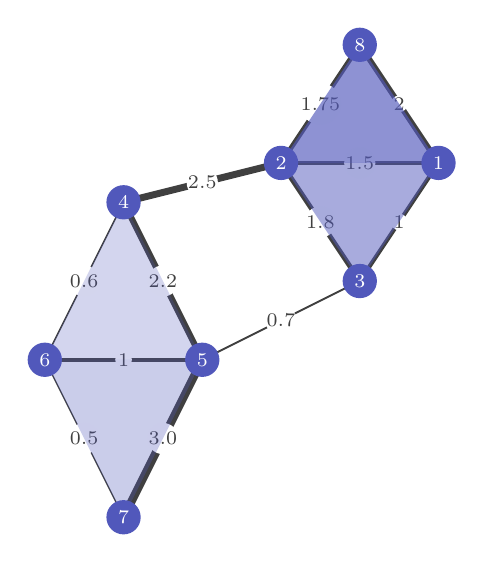
\begin{tikzpicture}
            \fill [opacity=0.25,liberty]    (0, 0) -- (2, 0) --  (1, 2) -- cycle;
             \fill [opacity=0.3,liberty]    (0, 0) -- (2, 0) --  (1, -2) -- cycle;
            \fill [opacity=0.5,liberty]    (4, 1) -- (3, 2.5) --  (5, 2.5) -- cycle;
            \fill [opacity=0.65,liberty]    (3, 2.5) -- (5, 2.5) --  (4, 4) -- cycle;
            \Vertex[x=0, y=0, style={color=liberty}, fontcolor=white, size=0.4, label = 6 ]{v1}
            \Vertex[x=2,y=0, style={color=liberty}, fontcolor=white, size=0.4, label = 5 ]{v2}
            \Vertex[x=1, y=2, style={color=liberty}, fontcolor=white, size=0.4, label=4]{v3}
            \Vertex[x=4, y=1, style={color=liberty}, fontcolor=white, size=0.4, label=3]{v4}
            \Vertex[x=3, y=2.5, style={color=liberty}, fontcolor=white, size=0.4, label=2]{v5}
            \Vertex[x=5, y=2.5, style={color=liberty}, fontcolor=white, size=0.4, label=1]{v6}
            \Vertex[x=4, y=4, style={color=liberty}, fontcolor=white, size=0.4, label=8]{v7}
            \Vertex[x=1, y=-2, style={liberty}, fontcolor=white, size = 0.4, label = 7]{v8}
            \Edge[Math, label=1](v1)(v2)
            \Edge[Math, label=0.6, lw=0.6pt](v1)(v3)
            \Edge[Math, label=2.2, lw=2.2pt](v2)(v3)
            \Edge[Math, label=0.7, lw=0.7](v2)(v4)
            \Edge[Math, label=2.5, lw=2.5](v3)(v5)
            \Edge[Math, label=1.8, lw=1.8](v4)(v5)
            \Edge[Math, label=1](v4)(v6)
            \Edge[Math, label=1.5, lw=1.5](v5)(v6)
            \Edge[Math, label=1.75, lw=1.75](v5)(v7)
            \Edge[Math, label=2, lw=2](v6)(v7)
            \Edge[Math, label=0.5,  lw =0.5pt](v1)(v8)
             \Edge[Math, label=3.0,  lw=3.0pt](v2)(v8)
        \end{tikzpicture}}
        \scalebox{0.7}{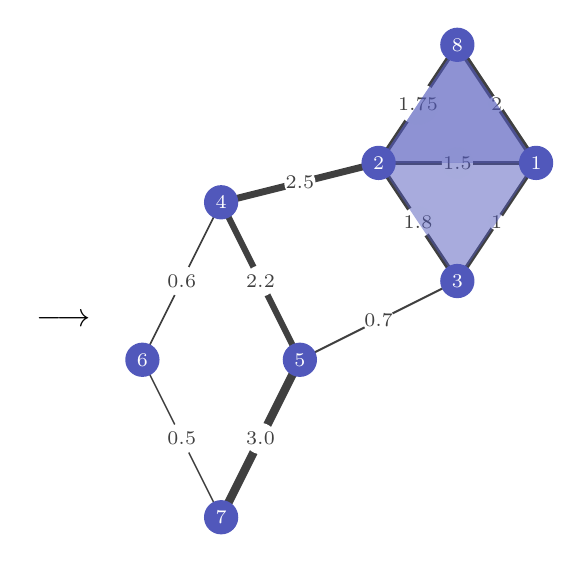
\begin{tikzpicture}
             \node at (-1, 0.5) {\large $\longrightarrow$};
            \fill [opacity=0.5,liberty]    (4, 1) -- (3, 2.5) --  (5, 2.5) -- cycle;
            \fill [opacity=0.65,liberty]    (3, 2.5) -- (5, 2.5) --  (4, 4) -- cycle;
            \Vertex[x=0, y=0, style={color=liberty}, fontcolor=white, size=0.4, label = 6 ]{v1}
            \Vertex[x=2,y=0, style={color=liberty}, fontcolor=white, size=0.4, label = 5 ]{v2}
            \Vertex[x=1, y=2, style={color=liberty}, fontcolor=white, size=0.4, label=4]{v3}
            \Vertex[x=4, y=1, style={color=liberty}, fontcolor=white, size=0.4, label=3]{v4}
            \Vertex[x=3, y=2.5, style={color=liberty}, fontcolor=white, size=0.4, label=2]{v5}
            \Vertex[x=5, y=2.5, style={color=liberty}, fontcolor=white, size=0.4, label=1]{v6}
            \Vertex[x=4, y=4, style={color=liberty}, fontcolor=white, size=0.4, label=8]{v7}
            \Vertex[x=1, y=-2, style={liberty}, fontcolor=white, size = 0.4, label = 7]{v8}
            %\Edge[Math, label=1](v1)(v2)
            \Edge[Math, label=0.6, lw=0.6pt](v1)(v3)
            \Edge[Math, label=2.2, lw=2.2pt](v2)(v3)
            \Edge[Math, label=0.7, lw=0.7](v2)(v4)
            \Edge[Math, label=2.5, lw=2.5](v3)(v5)
            \Edge[Math, label=1.8, lw=1.8](v4)(v5)
            \Edge[Math, label=1](v4)(v6)
            \Edge[Math, label=1.5, lw=1.5](v5)(v6)
            \Edge[Math, label=1.75, lw=1.75](v5)(v7)
            \Edge[Math, label=2, lw=2](v6)(v7)
            \Edge[Math, label=0.5,  lw =0.5pt](v1)(v8)
             \Edge[Math, label=3.0,  lw=3.0pt](v2)(v8)
        \end{tikzpicture}}
    \caption{
   % \brev
    Simplicial complex $\mc K$ on $8$ vertices for the illustrative run (on the left): all 2-simplices from $\mc V_2$ are shown in blue, the weight of each edge $w_1(e_i)$ is given on the figure. On the right: perturbed simplicial complex $\mc K$ through the elimination of the edge $[5,6]$ creating additional hole $[5, 6, 7, 8]$.
    \label{fig:illustrative_start}
    %\erev
    }
\end{figure}


\begin{figure}[t]
    \centering
    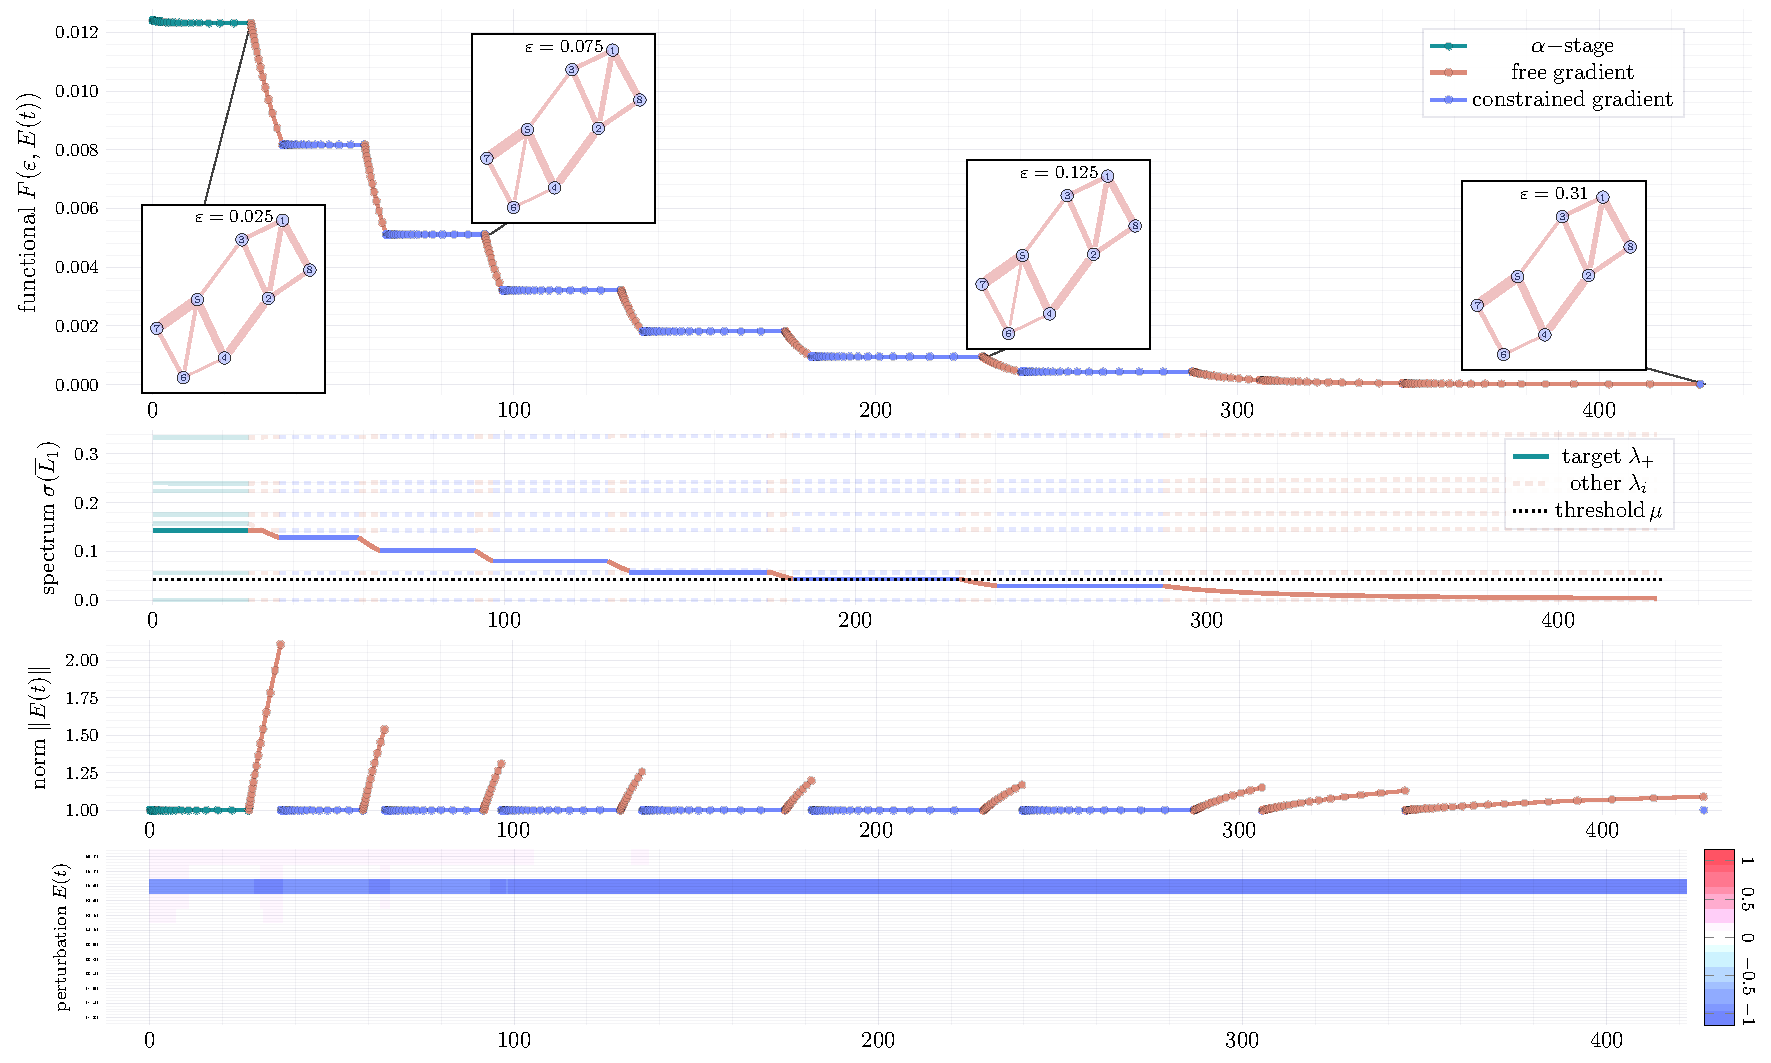
\includegraphics[width=1.0\textwidth,clip,trim=8pt 7pt 8pt 5pt]{figures/julia/test2.pdf}
    
    \caption{Illustrative run of the framework determining the topological stability: the top pane --- the flow of the functional $F(\eps, E(t))$; the second pane --- the flow of $\sigma(\bar L_1)$, $\lambda_+$ is highlighted; third pane --- the change of the perturbation norm $\| E(t) \|$; the bottom pane --- the heatmap of the perturbation profile $E(t)$.
     \label{fig:illustrative}
    }
\end{figure}

The exemplary run of the optimization framework in time is shown on Figure~\ref{fig:illustrative}.
The top panel of Figure~\ref{fig:illustrative} provides the continued flow of the target functional $F(\eps, E(t))$ consisting of the initial $\alpha$-phase (in green) and alternated constrained (in blue) and free gradient (in orange) stages. As stated above, $F(\eps, E(t))$ is strictly monotonic along the flow since the support of $\mathbb P_+$  does not change. Since the initial setup is not pathological with respect to the connectivity, the initial  $\alpha$-phase essentially reduces to a single constrained gradient flow and terminates after one run with $\alpha=\alpha_*$.  The constrained gradient stages are characterized by a slow changing $E(t)$, which is essentially due to the flow performing small adjustments to find the correct rotation on the unit sphere, whereas the free gradient stage quickly decreases the target functional.

The second panel shows the  behaviour of first non-zero eigenvalue $\lambda_+(\eps, E(t))$ (solid line) of $\bar L_1^{up}(\eps, E(t))$ dropping through the ranks of $\sigma(\bar L_1(\eps, E(t)))$ (semi-transparent); similar to the case of the target functional $F(\eps, E(t))$, $\lambda_+(\eps, E(t))$ monotonically decreases. The rest of the eigenvalues exhibit only minor changes, and the rapidly changing $\lambda_+$ successfully passes through the connectivity threshold $\mu$ (dotted line). 

The third and the fourth panels show the evolution of the norm of the perturbation $\| E(t) \|$ and the perturbation $E(t)$ itself, respectively.  The norm $\| E(t) \| $ is conserved during the constrained-gradient and the $\alpha$- stages; these stages correspond to the optimization of the perturbation shape, as shown by the small positive values at the beginning of the bottom panel which eventually vanish. During the free gradient integration the norm $\| E(t) \|$ increases, but the relative change of the norm declines with the growth of $\eps_i$ to avoid jumping over the smallest possible $\eps$. Finally, due to the simplicity of the complex, the  edge we want to eliminate, $56$, dominates the flow from the very beginning (see bottom panel); such a clear pattern persists only in small examples, whereas for large networks the perturbation profile is initially spread out among all the edges.


\subsection{Triangulation Benchmark}

To provide more insight into the computational behavior of the method, we synthesize here an almost planar 
graph dataset. Namely, we assume $N$ uniformly sampled vertices on the unit square with a network built by the Delaunay triangulation;  then, edges are randomly added or erased to obtain the sparsity $\nu$  (so that the graph has $\frac 12  \nu N(N-1)$ edges overall). An order-2 simplicial complex $\mc K=(\mc V_0,\mc V_1,\mc V_2)$  is then formed by letting $\mc V_0$ be the generated vertices, $\mc V_1$ the edges, and $\mc V_2$ every $3$-clique of the graph; edges' weights are sampled uniformly between $1/4$ and $3/4$, namely $w_1(e_i) \sim U [\frac{1}{4}, \frac{3}{4} ]$.


An  example of such triangulation is shown in Figure~\ref{fig:triang}; here $N=8$ and edges $[6, 8]$ and $[2, 7]$ were eliminated to achieve the desired sparsity.

\begin{figure}[t]
    \centering
    \subfloat[Example of Triangulation and Holes]{ \label{fig:triang}
        \scalebox{0.35}{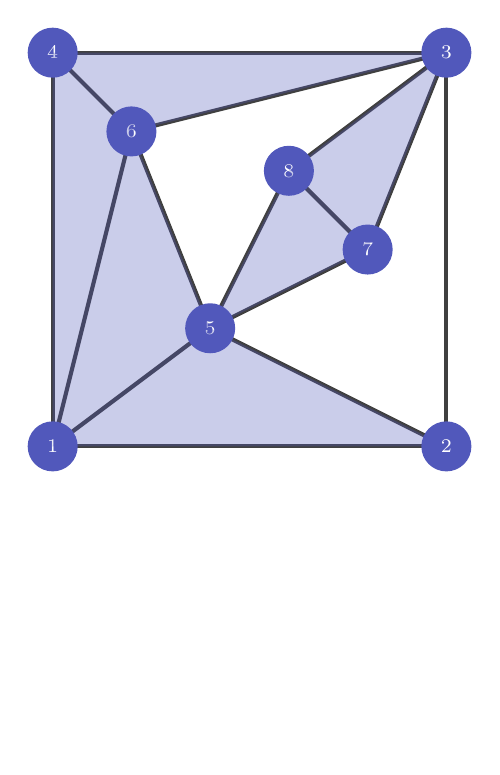
\begin{tikzpicture}
      \Vertex[x=0, y=0, label=1, style={color=liberty}, fontcolor=white,]{v1}
      \Vertex[x=5, y=0, label=2, style={color=liberty}, fontcolor=white,]{v2}
      \Vertex[x=5, y=5, label=3, style={color=liberty}, fontcolor=white,]{v3}
      \Vertex[x=0, y=5, label=4, style={color=liberty}, fontcolor=white,]{v4}
      \Vertex[x=2, y=1.5, label=5, style={color=liberty}, fontcolor=white,]{v5}
      \Vertex[x=1, y=4, label=6, style={color=liberty}, fontcolor=white,]{v6}
      \Vertex[x=4, y=2.5, label=7, style={color=liberty}, fontcolor=white,]{v7}
      \Vertex[x=3, y=3.5, label=8, style={color=liberty}, fontcolor=white,]{v8}
      \Edge(v1)(v2)
      \Edge(v2)(v3)
      \Edge(v3)(v4)
      \Edge(v1)(v4)
      \Edge(v1)(v5)
      \Edge(v2)(v5)
      %\Edge(v2)(v7)
      \Edge(v3)(v7)
      \Edge(v5)(v7)
      \Edge(v7)(v8)
      \Edge(v5)(v8)
      \Edge(v5)(v6)
      %\Edge(v6)(v8)
      \Edge(v3)(v8)
      \Edge(v4)(v6)
      \Edge(v1)(v6)
      \Edge(v3)(v6)

      \fill [opacity=0.3,liberty]   (v1.center) -- (v2.center) -- (v5.center) -- cycle;
      \fill [opacity=0.3,liberty]   (v1.center) -- (v4.center) -- (v6.center) -- cycle;
      \fill [opacity=0.3,liberty]   (v1.center) -- (v5.center) -- (v6.center) -- cycle;
      \fill [opacity=0.3,liberty]   (v3.center) -- (v4.center) -- (v6.center) -- cycle;
      \fill [opacity=0.3,liberty]   (v5.center) -- (v7.center) -- (v8.center) -- cycle;
      \fill [opacity=0.3,liberty]   (v3.center) -- (v7.center) -- (v8.center) -- cycle;
      
      \Vertex[x=0, y=-3.5, style={color=white}]{fake}
  \end{tikzpicture}}
    }
    \subfloat[Time (in seconds)]{\label{fig:triang_time}
       \scalebox{0.33}{%\input{times_prec2.tex}
        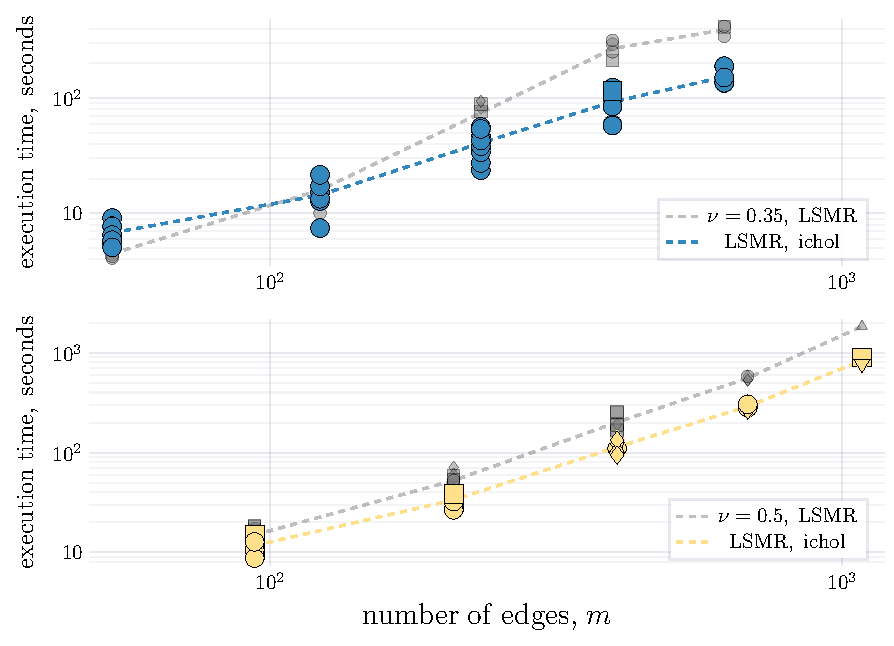
\includegraphics{figures/julia/times_prec2.pdf}
       }}
    \subfloat[Perturbation norm, $\eps$]{\label{fig:triang_eps}
        \scalebox{0.33}{%\input{eps_prec2.tex}
        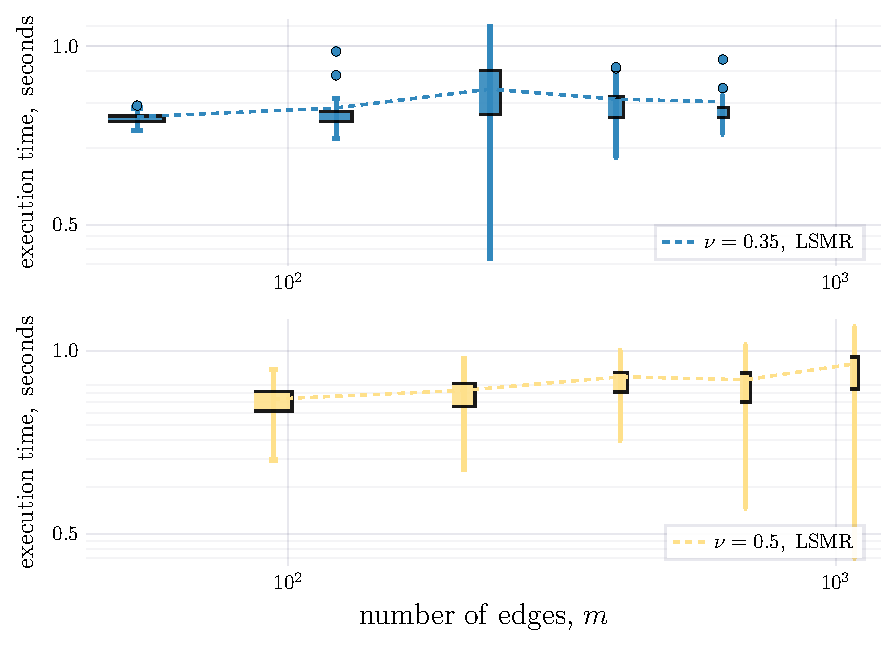
\includegraphics{figures/julia/eps_prec2.pdf}
        }}
        \caption{Benchmarking Results on the Synthetic Triangulation Dataset: varying sparsities $\nu=0.35, \, 0.5$ and $N=16, \, 22, \, 28, \, 34, \, 40$; each network is sampled $10$ times. Shapes correspond to the number of eliminated edges in the final perturbation: $1: \, \ocircle$, $2: \, \square$, $3: \pentagon$, $4: \, \triangle$. For each pair $(\nu, N)$, the un-preconditioned and Cholesky-preconditioned execution times are shown.}
        \vspace{-10pt}
\end{figure}

We sample networks with a varying number of vertices $N=10, \, 16, \, 22, \, 28$ and varying sparsity pattern $\nu=0.35, \, 0.5$ which determine the number of edges in the output  as $m = \nu \frac{N(N-1)}{2}$. Due to the highly randomized procedure, topological structures of a sampled graph with a fixed pair of parameters may differ substantially, so $10$ networks with the same $(N, \nu)$ pair are generated. For each network, the working time  (without considering the sampling itself) and the resulted perturbation norm $\eps$, and are reported in  Figure~\ref{fig:triang_time} and Figure~\ref{fig:triang_eps}, respectively. As anticipated in  Section~\ref{sec:computational_cost}, we show the performance of two implementations of the method, one based on LSMR and one based on LSMR preconditioned by using  the  incomplete Cholesky factorization of the initial matrices. We observe that, 
\begin{itemize}
    \item  the computational cost of the whole procedure  lies between $\mathcal O(m^2)$ and $\mathcal O(m^3)$ 
    \item denser structures, with a higher number of vertices, result in the higher number of edges being eliminated; at the same time, even most dense cases still can exhibit structures requiring the elimination of a single edge, showing that  the flow does not necessarily favor multi-edge optima;
    \item the required perturbation norm $\eps$ is growing with the size of the graph, Figure~\ref{fig:triang_eps}, but not too fast: it is expected that denser networks would require larger $\eps$ to create a new hole; at the same time if the perturbation were to grow drastically with the sparsity $\nu$, it would imply that the method tries to eliminate sufficiently more edges, a behavior that resembles convergence to a sub-optimal perturbation;
    \item preconditioning with a constant incomplete Cholesky multiplier, computed for the initial Laplacians, 
    provides a visible execution time gain for medium and large networks. Since the quality of the preconditioning deteriorates as the flow approaches the minimizer (as a non-zero eigenvalue becomes $0$), it is worth investigating the design of a preconditioner for the up-Laplacian that can be efficiently updated.
\end{itemize}


\subsection{Transportation Networks}

Finally, we provide an application to  real-world examples based on city transportation networks. 
We consider networks for Bologna, Anaheim, Berlin Mitte, and Berlin Tiergarten; each network consists of nodes --- intersections/public transport stops --- connected by edges (roads) and subdivided into zones; for each road the free flow time, length, speed limit are known; moreover, the travel demand for each pair of nodes is provided through the dataset of recorded trips.
All the datasets used here are publicly available at \url{https://github.com/bstabler/TransportationNetworks}; Bologna network is  provided by the Physic Department of the University of Bologna (enriched through the Google Maps API \url{https://developers.google.com/maps}).

The regularity of city maps naturally lacks $3$-cliques, hence forming the simplicial complex based on triangulations as done before frequently leads to trivial outcomes. 
Instead, here we ``lift'' the network to city zones, thus more effectively grouping the nodes in the graph. Specifically:
\begin{enumerate}
    \item we consider the completely connected graph where the nodes are zones in the city/region;
    \item the free flow time between two zones is temporarily assigned  as a weight of each edge: the time is as the shortest path between the zones (by the classic Dijkstra algorithm) 
    on the initial graph;
    \item similarly to what is done in the filtration used for persistent homology,  we filter out excessively distant nodes; additionally, we exclude the longest edges in each triangle in case it is equal to the sum of two other edges (so the triangle is degenerate and the trip by the longest edge is always performed through to others); 
    \item finally, we use the travel demand as an actual weight of the edges in the final network; travel demands are scaled \emph{logarithmically} via the transformation $w_i \mapsto \log_{10} \left(  \frac{w_i}{0.95 \min w_i} \right)$; see the example on the left panel of Figure~\ref{fig:bologna}.
\end{enumerate}
Given the definition of weights in the network, high instability (corresponding to small perturbation norm $\eps$) implies structural phenomena around the ``almost-hole'', where the faster and shorter route is sufficiently less demanded. 

\begin{figure}
    \centering
    \scalebox{1.0}[0.9]{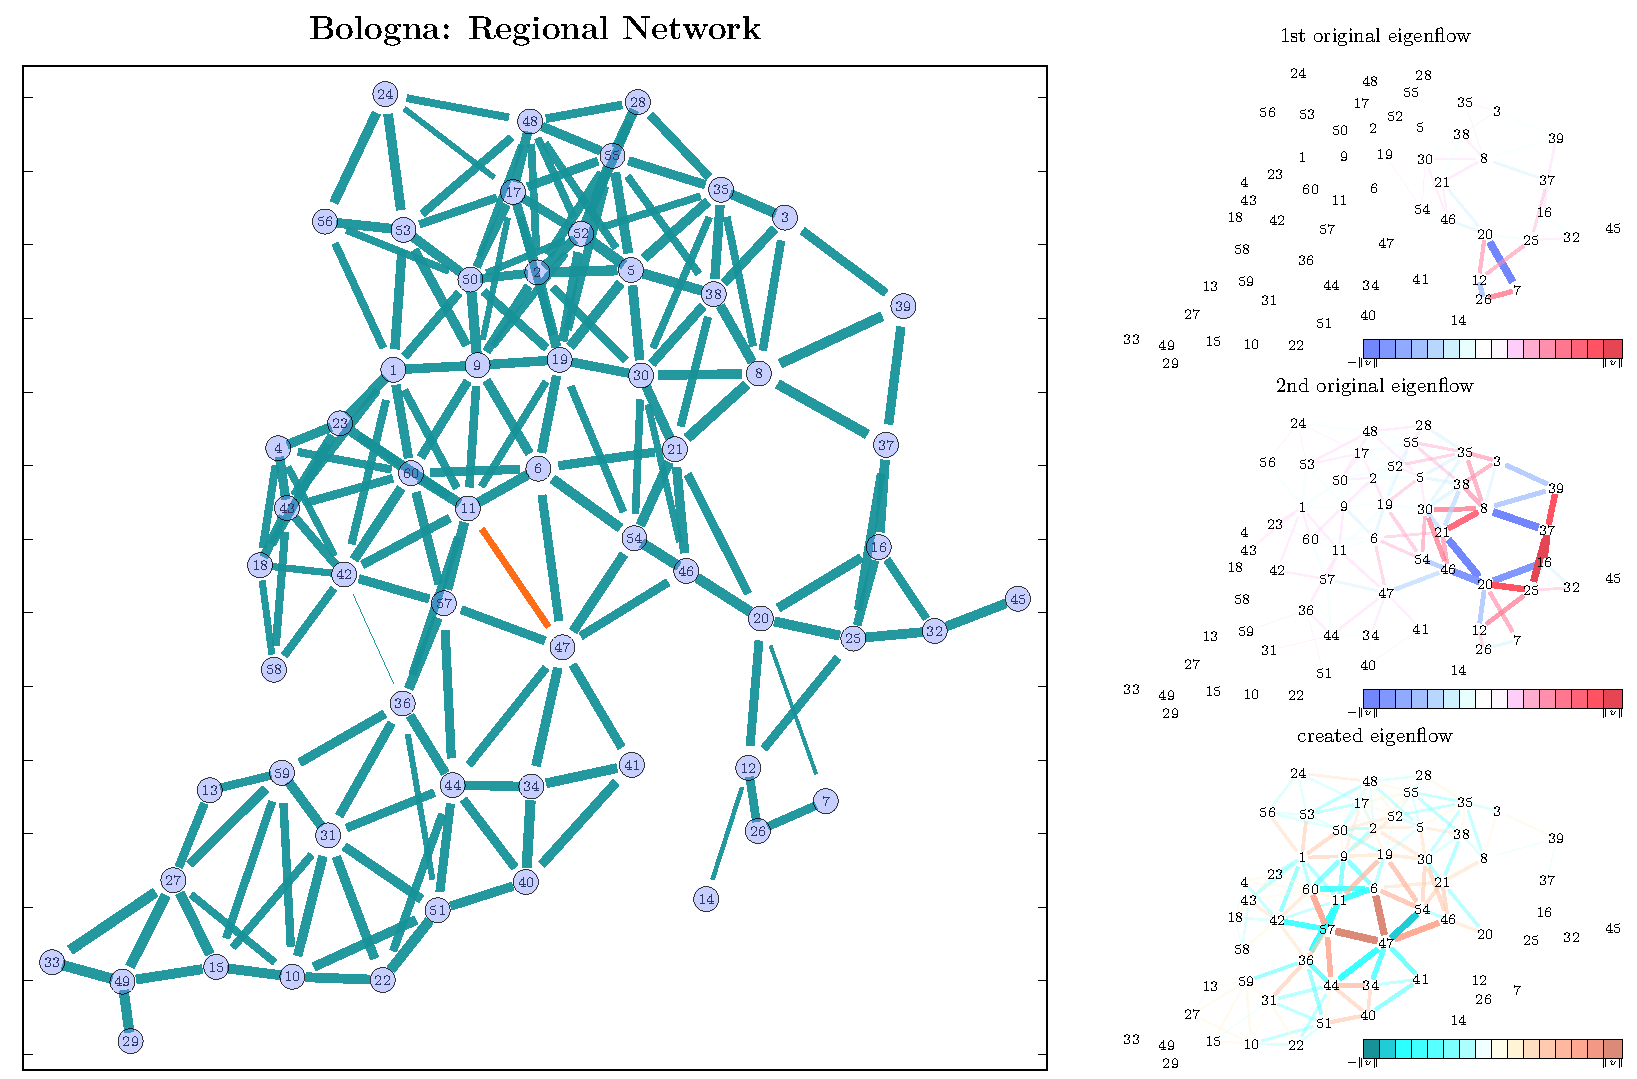
\includegraphics[width=1.0\columnwidth]{figures/julia/bologna.pdf}}
    \caption{Example of the Transportation Network for Bologna. Left pane: original zone graph where the width of edges corresponds to the weight, to-be-eliminated edge is colored in red. Right pane: eigenflows, original and created; color and width correspond to the magnitude of entries.}
    \label{fig:bologna}
\end{figure}


\begin{table}[hbtp]
  \centering
  \begin{NiceTabular}{@{}c!{\qquad}cccc!{\qquad}ccc@{}}
    \toprule
    \Block{2-1}{\bfseries Cities} & \Block{1-3}{\bfseries network} & & & \Block{2-1}{ \( \beta_1 \) } & \Block{1-3}{\bfseries logarithmic weights} \\
    & \( m_0 \) & \( m_1 \) & \( m_2 \) & & time & \( \eps \) & \( p \) \\
    \midrule
    \Block{2-1}{Bologna} & \Block{2-1}{60} & \Block{2-1}{175} & \Block{2-1}{171} & \Block{2-1}{2} &  \( 2.43 \)s & \( 0.65 \) & \( 0.003 \)\\
     &  &  &  & & \Block{1-3}{\small  \textbf{{[}11, 47{]}} ($4^{th}$ smallest) } \\[0.1cm]
     \dashedline
     \noalign{\vskip 0.1cm}
     \Block{2-1}{Anaheim} & \Block{2-1}{38} & \Block{2-1}{159} & \Block{2-1}{221} & \Block{2-1}{1} &  \( 5.39 \)s & \( 0.57 \) & \(0.003\)\\
     &  &  &  &  & \Block{1-3}{\small \textbf{{[}10, 29{]}} ($11^{th}$ smallest)} \\[0.1cm]
     \dashedline
     \noalign{\vskip 0.1cm}
     \Block{2-1}{Berlin-Tiergarten} & \Block{2-1}{26} & \Block{2-1}{63} & \Block{2-1}{55} & \Block{2-1}{0} & \(2.46\)s & \(1.18\) & \(0.015\) \\
     & &  & & & \Block{1-3}{\small \textbf{{[}6, 16{]}} ($20^{th}$ smallest)} \\[0.1cm]
     \dashedline
     \noalign{\vskip 0.1cm}
     \Block{2-1}{Berlin-Mitte} & \Block{2-1}{98} & \Block{2-1}{456} & \Block{2-1}{900} & \Block{2-1}{1} &  \( 127 \)s & \(0.887\) & \(0.0016\)\\
     & & & & & \Block{1-3}{\small \textbf{{[}57, 87{]}} ($6^{th}$), \textbf{{[}58, 87{]}}, ($17^{th}$) } \\
    \bottomrule
    \end{NiceTabular}

    \caption{
      Topological instability of the transportation networks: filtered zone networks with the corresponding perturbation norm \( \eps \) and its percentile among \( w_1(\cdot) \) profile. For each simplicial complex the number of nodes, edges and triangles in \( \mc V_2(\mc K) \) are provided alongside the initial number of holes \( \beta_1 \). The results of the algorithm consist of the perturbation norm, \( \eps \), computation time, and approximate percentile \( p \).\label{tab:bologna}
    }
  
\end{table}

In the case of Bologna, Figure~\ref{fig:bologna}, the algorithm eliminates the edge $[11, 47]$ (Casalecchio di Reno -- Pianoro) creating a new hole $6 - 11 - 57 - 47$. We also provide examples of the eigenflows in the kernel of the Hodge Laplacian (original and additional perturbed): original eigenvectors correspond to the circulations around holes $7-26-12-20$ and $8-21-20-16-37$ non-locally spread in the neighborhood~\cite{schaub2020random}. 

The results for four different networks are summarized in the Table~\ref{tab:bologna}; $p$ mimics the percentile, $\eps/\sum_{e\in \mc V_1}{w_i(e)}$, showing the overall small perturbation norm contextually. 
At the same time, we emphasize that except Bologna (which is influenced by the geographical topology of the land), the algorithm does not choose the smallest weight possible; indeed, given our interpretation of the topological instability, the complex for Berlin-Tiergarten is stable and the transportation network is effectively constructed.

































\chapter{Topological Stability of Simplicial Complexes}
\section{Preconditioning}

\begin{tmp}
      Here we need to say general words about how we need an efficient preconditioning scheme.
\end{tmp}

\subsection{Preconditioning 101}

\subsection{Cholesky preconditioning for classical graphs}

\subsection{Classical collapsibility}

% TODO: introduction


In this section we borrow the terminology from \cite{whiteheadSimplicialSpacesNuclei1939}; additionally, let us  assume that considered simplicial complex \( \mc K \) is restricted to its \(2\)-skeleton, so \( \mc K \) consists only of nodes, edges, and triangles, \( \mc K = \V 0 \cup \V 1 \cup \V 2\).

Simplex \( \tau \in \mc K \) is called an (inlusion-wise) \gls{maximal face} of simplex \( \sigma \in \mc K \) if \( \tau \) is maximal by inlusion simplex such that \( \sigma \subseteq \tau \) and \( \ord \sigma < \ord \tau \). \en{
      \insidefigure[0.3\columnwidth]{\begin{tikzpicture}

      \fill [opacity=0.5,liberty]    (0, 0) -- (2, 0) --  (1, 1.5) -- cycle;
      \fill [opacity=0.3,liberty]    (0, 0) -- (2, 0) --  (1, -1.5) -- cycle;

      \Vertex[x=0, y=0, style={color=persimmon}, fontcolor=white, size=0.2, label = 1]{v1}
      \Vertex[x=2, y=0, style={color=persimmon}, fontcolor=white, size=0.2, label = 2]{v2}
      \Vertex[x=1, y=1.5, style={color=persimmon}, fontcolor=white, size=0.2, label = 3]{v3}
      \Vertex[x=1, y=-1.5, style={color=persimmon}, fontcolor=white, size=0.2, label = 4]{v4}

      \Edge[](v1)(v2)
      \Edge[](v1)(v3)
      \Edge[](v2)(v3)
      \Edge[](v1)(v4)
      \Edge[](v2)(v4)


\end{tikzpicture}}{Example of a simplicial complex: free simplices and maximal faces. \label{fig:adjacent_triangles}}
} For instance, in \Cref{fig:adjacent_triangles} the edge \( \{1, 2\} \) and nodes \( \{ 1 \} \) and \( \{ 2 \} \) have two maximal faces, \( \{ 1, 2, 3 \} \) and \( \{ 1, 2, 4 \} \), while all the other edges and nodes have unique maximal faces --- their corresponding triangles. Note that in the case of the node \( \{ 1 \} \), there are bigger simplices containing it besides the triangles (e.g. the edge \( \{ 1, 2 \} \)), but they are not maximal by inclusion.

\begin{definition}[Free simplex]\label{def:free}
      The simplex \(\sigma \in \mc K \) is \gls{free} if it has exactly one maximal face \( \tau \), \( \tau = \tau(\sigma) \). F.i. edges \( \{ 1, 3 \} \), \( \{ 1, 4 \} \), \( \{ 2, 3 \} \) and \( \{ 2, 4 \} \) are all free in \Cref{fig:adjacent_triangles}.
\end{definition} 

 The \gls{collapse} \( \mc K \backslash \{ \sigma \} \) of \( \mc K \) at a free simplex \( \sigma \) is the transition from the original simplicial complex \( \mc K \) to a smaller simplicial complex \( \mc L \) without the free simplex \( \sigma \) and the corresponding maximal face \( \tau \), \( \mc K \to \mc K' = \mc K - \sigma - \tau \); namely, one can eliminate a simplex \( \tau \) if it has an accessible (not included in another simplex) face \(\sigma\).

Naturally, one can perform several consequent collapses at  \( \Sigma = \{ \sigma_1, \sigma_2, \ldots \} \) assuming \( \sigma_i \) is free in collapse simplicial complex from the previous stage; \( \Sigma \) is called the \gls{collapsing sequence}. Formally:
 \begin{definition}[Collapsing sequence]
       Let \( \mc K \) be a simplicial complex. \( \Sigma = \{ \sigma_1, \sigma_2, \ldots \} \) is a \gls{collapsing sequence} if \( \sigma_1 \) is free in \( \mc K \) and each \( \sigma_i \), \( i > 1 \), is free at 
       \( \mc K^{(i)} = \mc K^{(i-1)} \backslash \{ \sigma_i \} \), \( \mc K^{(1)} = \mc K \). The collapse of \( \mc K \) to a new complex \( \mc L \) at \( \Sigma \) is denoted by \( \mc L = \mc K \backslash \Sigma \).
 \end{definition}
 By the definition, every collapsing sequence \( \Sigma \) has a corresponding sequence \( \ds T = \{ \tau(\sigma_1), \tau(\sigma_2), \ldots \} \) of maximal faces being collapsed at every step.

 \begin{definition}[Collapsible simplicial complex, \cite{whiteheadSimplicialSpacesNuclei1939}]
      The simplicial complex \( \mc K \) is \gls{collapsible} if there exists a collapsing sequence \( \Sigma \) such that \( \mc K \) collapses to a single vertex at \( \Sigma \), \( \mc K \backslash \Sigma = \{ v \} \).
\end{definition}

Determining whether the complex is collapsible is in general \emph{NP-complete},~\cite{tancerRecognitionCollapsibleComplexes2016}, but can be almost linear for a set of specific families of \( \mc K \), e.g.\ if the simplex can be embeded into the triangulation of the \(d\)-dimensional unit sphere,~\cite{cohenSolving1laplaciansNearly2014}. Naturally restricting the collapses to the case of \(d\)-collapses (such that \( \ord \sigma_i \le d-1 \)), one arrive at the notion of \(d\)-collapsibility,~\cite{tancerDcollapsibilityNPcomplete2009}.

\begin{definition}[\(d\)-Core]
      A \(d\)-Core is a subcomplex of \( \mc K \) such that every simplex of order \( d - 1\) belongs to at least \( 2 \) simplices of order \( d \). E.g. \(2\)-Core is such a subcomplex of the original 2-skeleton \( \mc K \) that every edge from \( \V 1 \) belong to at least \(2\) triangles from \( \V 2 \).
\end{definition}

\begin{lemma}[\cite{lofanoWorstWayCollapse2021}]
      \( \mc K \) is \(d\)-collapsible if and only if it does not contain a \( d\)-core.
\end{lemma}
\begin{proof}
      The proof of the lemma above naturally follows from the definition of the core. Assume \( \Sigma \) is a \(d\)-collapsing sequence, and \( \mc K \backslash \Sigma \) consists of more than a single vertex and has no free simplices of order \( \le d-1\) (``collapsing sequence gets stuck''). Then, each simplex of order \( d-1 \) is no free but belongs to at least \(2\) simplices of order \(d\), so \( \mc K \backslash \Sigma \) is a \( d \)-Core. 
      
      Conversely if a \(d\)-Core exists in the complex, the collapsing sequence should necessarily include its simplices of order \( d - 1 \) which can not become free during as a result of a sequence of collapses. Indeed, for \(\sigma\) from \(d\)-Core,  \(\ord \sigma = d-1\), to become free, one needs to collapse at least one of \(\sigma\)'s maximal faces for \( d\)-Core , all of whose faces are, in turn, contained in the \( d\)-Core (since \(d\)-Core is a simplicial complex). As a result one necessarily needs a prior collapse inside the \(d\)-Core to perform the first collapse in the \(d\)-Core, which is impossible. 
\end{proof}

In the case of the classical graph model, the \( 1 \)-Core is a subgraph where each vertex has a degree at least \( 2 \); in other words, \( 1 \)-Core cannot be a tree and necessarily contains a simple cycle. Hence, the collapsibility of a classical graph coincides with the acyclicity. The \(d\)-Core is the generalization of the cycle for the case of \(1\)-collapsibility of the classical graph; additionally, the \(d\)-Core is very dense due to its definition. In the case of \(2\)-Core, we provide simple exemplary structures on \Cref{fig:2-core} which imply various possible configurations for a  \(d\)-Core, \( d \ge 2 \), hence a search for \(d\)-Core inside \( \mc K \) is neither trivial, no computationally cheap.

\begin{figure}[htbp]
      \centering
      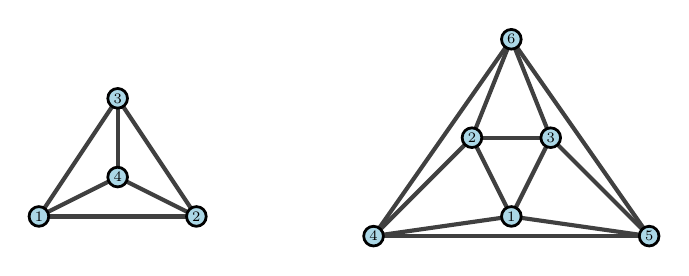
\begin{tikzpicture}
      \Vertex[x=0, y=0, size=0.25, fontscale=0.75, label=1]{v1}
      \Vertex[x=2, y=0, size=0.25, fontscale=0.75,label=2]{v2}
      \Vertex[x=1, y=1.5, size=0.25,fontscale=0.75, label=3]{v3}
      \Vertex[x=1, y=0.5, size=0.25,fontscale=0.75, label=4]{v4} 
      \Edge(v1)(v2)
      \Edge(v1)(v3)
      \Edge(v1)(v4)
      \Edge(v2)(v3)
      \Edge(v2)(v4)
      \Edge(v3)(v4)

      
      \Vertex[x=6, y=0, size=0.25, fontscale=0.75, label=1]{v1}
      \Vertex[x=5.5, y=1, size=0.25, fontscale=0.75, label=2]{v2}
      \Vertex[x=6.5, y=1, size=0.25, fontscale=0.75, label=3]{v3}
      \Vertex[x=4.25, y=-0.25, size=0.25, fontscale=0.75, label=4]{v4}
      \Vertex[x=7.75, y=-0.25, size=0.25, fontscale=0.75, label=5]{v5}
      \Vertex[x=6, y=2.25, size=0.25, fontscale=0.75, label=6]{v6}
      \Edge(v1)(v2)
      \Edge(v2)(v3)
      \Edge(v1)(v3)
      \Edge(v4)(v5)
      \Edge(v4)(v6)
      \Edge(v5)(v6)
      \Edge(v1)(v4)
      \Edge(v1)(v5)
      \Edge(v2)(v6)
      \Edge(v3)(v6)
      \Edge(v2)(v4)
      \Edge(v3)(v5)
\end{tikzpicture}
      \caption{ \(2\)-Core, examples. \label{fig:2-core} }
\end{figure}

%Besides the quantitative restriction discussed later, \( 2 \)-Cores tend to appear relatively early when upon ``densifying'' the complex.
Additionally, we demonstrate that an arbitrary simplicial complex \(\mc K\) tends to contain \(2\)-Cores as long as \( \mc K \) is denser than a trivially collapsible case. Assume the complex formed by triangulation of \( m_0 \) random points on the unit square with a sparsity pattern \( \nu \); the triangulation itself with the corresponding \( \nu_\Delta \) is collapsible, but a reasonably small addition of edges already creates a \(2\)-Core (since it is local), \Cref{fig:core_prob}, left. Similarly, sampled sensor networks, where \( \exists \sigma \in \V 1: \; \sigma = [v_1, v_2] \iff \| v_1 - v_2 \|_2 < \eps \) for a chosen percolation parameter \( \eps > 0 \), quickly form a 2-Core upon the densifying of the network.

\begin{figure}[htbp]
      \centering
      \scalebox{0.4}{
            % Recommended preamble:
% \usetikzlibrary{arrows.meta}
% \usetikzlibrary{backgrounds}
% \usepgfplotslibrary{patchplots}
% \usepgfplotslibrary{fillbetween}
% \pgfplotsset{%
%     layers/standard/.define layer set={%
%         background,axis background,axis grid,axis ticks,axis lines,axis tick labels,pre main,main,axis descriptions,axis foreground%
%     }{
%         grid style={/pgfplots/on layer=axis grid},%
%         tick style={/pgfplots/on layer=axis ticks},%
%         axis line style={/pgfplots/on layer=axis lines},%
%         label style={/pgfplots/on layer=axis descriptions},%
%         legend style={/pgfplots/on layer=axis descriptions},%
%         title style={/pgfplots/on layer=axis descriptions},%
%         colorbar style={/pgfplots/on layer=axis descriptions},%
%         ticklabel style={/pgfplots/on layer=axis tick labels},%
%         axis background@ style={/pgfplots/on layer=axis background},%
%         3d box foreground style={/pgfplots/on layer=axis foreground},%
%     },
% }

\begin{tikzpicture}[/tikz/background rectangle/.style={fill={rgb,1:red,1.0;green,1.0;blue,1.0}, draw opacity={1.0}}, show background rectangle]
      \begin{axis}[point meta max={nan}, point meta min={nan}, legend cell align={left}, legend columns={1}, title={}, title style={at={{(0.5,1)}}, anchor={south}, font={{\fontsize{18 pt}{23.400000000000002 pt}\selectfont}}, color={rgb,1:red,0.0;green,0.0;blue,0.0}, draw opacity={1.0}, rotate={0.0}, align={center}}, legend style={color={rgb,1:red,0.1333;green,0.1333;blue,0.3333}, draw opacity={0.1}, line width={1}, solid, fill={rgb,1:red,1.0;green,1.0;blue,1.0}, fill opacity={0.9}, text opacity={1.0}, font={{\fontsize{22 pt}{28.6 pt}\selectfont}}, text={rgb,1:red,0.0;green,0.0;blue,0.0}, cells={anchor={center}}, at={(0.98, 0.02)}, anchor={south east}}, axis background/.style={fill={rgb,1:red,1.0;green,1.0;blue,1.0}, opacity={1.0}}, anchor={north west}, xshift={1.0mm}, yshift={-1.0mm}, width={150.4mm}, height={150.4mm}, scaled x ticks={false}, xlabel={$\mathrm{sparsity \; (wrt \; triangulation)}$}, x tick style={draw={none}}, x tick label style={color={rgb,1:red,0.0;green,0.0;blue,0.0}, opacity={1.0}, rotate={0}}, xlabel style={at={(ticklabel cs:0.5)}, anchor=near ticklabel, at={{(ticklabel cs:0.5)}}, anchor={near ticklabel}, font={{\fontsize{22 pt}{28.6 pt}\selectfont}}, color={rgb,1:red,0.0;green,0.0;blue,0.0}, draw opacity={1.0}, rotate={0.0}}, xmode={log}, log basis x={10}, xmajorgrids={true}, xmin={0.993342357875681}, xmax={1.2577738078862484}, xticklabels={{$\nu_\Delta$,$1.1\nu_\Delta$,$1.25\nu_\Delta$}}, xtick={{1.0,1.1,1.25}}, xtick align={inside}, xticklabel style={font={{\fontsize{18 pt}{23.400000000000002 pt}\selectfont}}, color={rgb,1:red,0.0;green,0.0;blue,0.0}, draw opacity={1.0}, rotate={0.0}}, x grid style={color={rgb,1:red,0.1333;green,0.1333;blue,0.3333}, draw opacity={0.1}, line width={0.5}, solid}, extra x ticks={{}}, extra x tick labels={}, extra x tick style={grid={major}, x grid style={color={rgb,1:red,0.1333;green,0.1333;blue,0.3333}, draw opacity={0.05}, line width={0.5}, solid}, major tick length={0}}, x axis line style={{draw opacity = 0}}, scaled y ticks={false}, ylabel={$\mathrm{probability \; of \; 2-Core}$}, y tick style={draw={none}}, y tick label style={color={rgb,1:red,0.0;green,0.0;blue,0.0}, opacity={1.0}, rotate={0}}, ylabel style={at={(ticklabel cs:0.5)}, anchor=near ticklabel, at={{(ticklabel cs:0.5)}}, anchor={near ticklabel}, font={{\fontsize{22 pt}{28.6 pt}\selectfont}}, color={rgb,1:red,0.0;green,0.0;blue,0.0}, draw opacity={1.0}, rotate={0.0}}, ymode={log}, log basis y={10}, ymajorgrids={true}, ymin={0.23981602983131609}, ymax={1.0424657608411214}, yticklabels={{$0.25$,$0.5$,$1$}}, ytick={{0.25,0.5,1.0}}, ytick align={inside}, yticklabel style={font={{\fontsize{18 pt}{23.400000000000002 pt}\selectfont}}, color={rgb,1:red,0.0;green,0.0;blue,0.0}, draw opacity={1.0}, rotate={0.0}}, y grid style={color={rgb,1:red,0.1333;green,0.1333;blue,0.3333}, draw opacity={0.1}, line width={0.5}, solid}, extra y ticks={{}}, extra y tick labels={}, extra y tick style={grid={major}, y grid style={color={rgb,1:red,0.1333;green,0.1333;blue,0.3333}, draw opacity={0.05}, line width={0.5}, solid}, major tick length={0}}, y axis line style={{draw opacity = 0}}, colorbar={false}]
          \addplot[color={rgb,1:red,0.8;green,0.4;blue,0.4667}, name path={393a1deb-0ad5-49fa-841c-c2d680cf69bc}, draw opacity={1.0}, line width={1.2}, solid, mark={*}, mark size={4.5 pt}, mark repeat={1}, mark options={color={rgb,1:red,0.0;green,0.0;blue,0.0}, draw opacity={1.0}, fill={rgb,1:red,0.8;green,0.4;blue,0.4667}, fill opacity={1.0}, line width={0.0}, rotate={0}, solid}]
              table[row sep={\\}]
              {
                  \\
                  1.009246153846154  0.25  \\
                  1.0134923076923077  0.25  \\
                  1.0177384615384615  0.25  \\
                  1.0219846153846153  0.25  \\
                  1.0262307692307693  0.41  \\
                  1.030476923076923  0.41  \\
                  1.0347230769230769  0.41  \\
                  1.0389692307692306  0.558  \\
                  1.0432153846153847  0.558  \\
                  1.0474615384615384  0.558  \\
                  1.0517076923076922  0.558  \\
                  1.0559538461538462  0.674  \\
                  1.0602  0.674  \\
                  1.0644461538461538  0.674  \\
                  1.0686923076923076  0.674  \\
                  1.0729384615384616  0.758  \\
                  1.0771846153846154  0.758  \\
                  1.0814307692307692  0.758  \\
                  1.0856769230769232  0.846  \\
                  1.089923076923077  0.846  \\
                  1.0941692307692308  0.846  \\
                  1.0984153846153846  0.846  \\
                  1.1026615384615386  0.898  \\
                  1.1069076923076924  0.898  \\
                  1.1111538461538462  0.898  \\
                  1.1154  0.94  \\
                  1.119646153846154  0.94  \\
                  1.1238923076923077  0.94  \\
                  1.1281384615384615  0.94  \\
                  1.1323846153846155  0.958  \\
                  1.1366307692307693  0.958  \\
                  1.1408769230769231  0.958  \\
                  1.145123076923077  0.958  \\
                  1.149369230769231  0.974  \\
                  1.1536153846153847  0.974  \\
                  1.1578615384615385  0.974  \\
                  1.162107692307692  0.988  \\
                  1.166353846153846  0.988  \\
                  1.1705999999999999  0.988  \\
                  1.1748461538461537  0.988  \\
                  1.1790923076923077  0.994  \\
                  1.1833384615384615  0.994  \\
                  1.1875846153846152  0.994  \\
                  1.191830769230769  0.994  \\
                  1.196076923076923  0.998  \\
                  1.2003230769230768  0.998  \\
                  1.2045692307692306  0.998  \\
                  1.2088153846153846  1.0  \\
                  1.2130615384615384  1.0  \\
                  1.2173076923076922  1.0  \\
                  1.221553846153846  1.0  \\
                  1.2258  1.0  \\
                  1.2300461538461538  1.0  \\
                  1.2342923076923076  1.0  \\
                  1.2385384615384614  1.0  \\
                  1.2427846153846154  1.0  \\
                  1.2470307692307692  1.0  \\
              }
              ;
          \addlegendentry {$\mathcal{V}_0(\mathcal K)=24$}
          \addplot[color={rgb,1:red,0.2;green,0.1333;blue,0.5333}, name path={3388d577-df0a-4b0f-bb98-8e4a3883b6b4}, draw opacity={1.0}, line width={1.2}, solid, mark={*}, mark size={4.5 pt}, mark repeat={1}, mark options={color={rgb,1:red,0.0;green,0.0;blue,0.0}, draw opacity={1.0}, fill={rgb,1:red,0.2;green,0.1333;blue,0.5333}, fill opacity={1.0}, line width={0.0}, rotate={0}, solid}]
              table[row sep={\\}]
              {
                  \\
                  1.0153999999999999  0.476  \\
                  1.0179999999999998  0.476  \\
                  1.0206  0.476  \\
                  1.0231999999999999  0.476  \\
                  1.0257999999999998  0.476  \\
                  1.0283999999999998  0.476  \\
                  1.031  0.476  \\
                  1.0335999999999999  0.476  \\
                  1.0361999999999998  0.476  \\
                  1.0388  0.476  \\
                  1.0413999999999999  0.476  \\
                  1.0439999999999998  0.8  \\
                  1.0466  0.8  \\
                  1.0492  0.8  \\
                  1.0517999999999998  0.8  \\
                  1.0543999999999998  0.8  \\
                  1.057  0.8  \\
                  1.0595999999999999  0.8  \\
                  1.0621999999999998  0.8  \\
                  1.0648  0.8  \\
                  1.0674  0.8  \\
                  1.0699999999999998  0.8  \\
                  1.0726  0.916  \\
                  1.0752  0.916  \\
                  1.0777999999999999  0.916  \\
                  1.0803999999999998  0.916  \\
                  1.083  0.916  \\
                  1.0856  0.916  \\
                  1.0881999999999998  0.916  \\
                  1.0908  0.916  \\
                  1.0934  0.916  \\
                  1.0959999999999999  0.916  \\
                  1.0986  0.916  \\
                  1.1011999999999997  0.972  \\
                  1.1037999999999997  0.972  \\
                  1.1063999999999998  0.972  \\
                  1.1089999999999998  0.972  \\
                  1.1115999999999997  0.972  \\
                  1.1141999999999999  0.972  \\
                  1.1167999999999998  0.972  \\
                  1.1193999999999997  0.972  \\
                  1.1219999999999999  0.972  \\
                  1.1245999999999998  0.972  \\
                  1.1271999999999998  0.972  \\
                  1.1297999999999997  0.986  \\
                  1.1323999999999999  0.986  \\
                  1.1349999999999998  0.986  \\
                  1.1375999999999997  0.986  \\
                  1.1401999999999999  0.986  \\
                  1.1427999999999998  0.986  \\
                  1.1453999999999998  0.986  \\
                  1.148  0.986  \\
                  1.1505999999999998  0.986  \\
                  1.1531999999999998  0.986  \\
                  1.1557999999999997  0.986  \\
                  1.1583999999999999  0.998  \\
                  1.1609999999999998  0.998  \\
                  1.1635999999999997  0.998  \\
                  1.1662  0.998  \\
                  1.1687999999999998  0.998  \\
                  1.1713999999999998  0.998  \\
                  1.174  0.998  \\
                  1.1765999999999999  0.998  \\
                  1.1791999999999998  0.998  \\
                  1.1817999999999997  0.998  \\
                  1.1844  0.998  \\
                  1.1869999999999998  1.0  \\
                  1.1895999999999998  1.0  \\
                  1.1922  1.0  \\
                  1.1947999999999999  1.0  \\
                  1.1973999999999998  1.0  \\
                  1.2  1.0  \\
                  1.2026  1.0  \\
                  1.2051999999999998  1.0  \\
                  1.2077999999999998  1.0  \\
                  1.2104  1.0  \\
                  1.2129999999999999  1.0  \\
                  1.2155999999999998  1.0  \\
                  1.2182  1.0  \\
                  1.2207999999999999  1.0  \\
                  1.2233999999999998  1.0  \\
                  1.226  1.0  \\
                  1.2286  1.0  \\
                  1.2311999999999999  1.0  \\
                  1.2337999999999998  1.0  \\
                  1.2363999999999997  1.0  \\
                  1.2389999999999997  1.0  \\
                  1.2415999999999998  1.0  \\
                  1.2441999999999998  1.0  \\
                  1.2467999999999997  1.0  \\
                  1.2493999999999998  1.0  \\
              }
              ;
          \addlegendentry {$\mathcal{V}_0(\mathcal K)=14$}
          \addplot[color={rgb,1:red,0.8667;green,0.8;blue,0.4667}, name path={51c0f6ce-ed32-4088-b026-cb9827a330bb}, draw opacity={1.0}, line width={1.2}, solid, mark={*}, mark size={4.5 pt}, mark repeat={1}, mark options={color={rgb,1:red,0.0;green,0.0;blue,0.0}, draw opacity={1.0}, fill={rgb,1:red,0.8667;green,0.8;blue,0.4667}, fill opacity={1.0}, line width={0.0}, rotate={0}, solid}]
              table[row sep={\\}]
              {
                  \\
                  1.0118399999999999  0.33  \\
                  1.01526  0.33  \\
                  1.01868  0.33  \\
                  1.0221  0.33  \\
                  1.02552  0.33  \\
                  1.02894  0.33  \\
                  1.03236  0.556  \\
                  1.03578  0.556  \\
                  1.0392  0.556  \\
                  1.0426199999999999  0.556  \\
                  1.04604  0.556  \\
                  1.04946  0.556  \\
                  1.05288  0.706  \\
                  1.0563  0.706  \\
                  1.05972  0.706  \\
                  1.06314  0.706  \\
                  1.06656  0.706  \\
                  1.06998  0.706  \\
                  1.0734  0.812  \\
                  1.07682  0.812  \\
                  1.08024  0.812  \\
                  1.08366  0.812  \\
                  1.08708  0.812  \\
                  1.0905  0.892  \\
                  1.09392  0.892  \\
                  1.09734  0.892  \\
                  1.10076  0.892  \\
                  1.10418  0.892  \\
                  1.1076  0.892  \\
                  1.11102  0.934  \\
                  1.1144399999999999  0.934  \\
                  1.1178599999999999  0.934  \\
                  1.1212799999999998  0.934  \\
                  1.1246999999999998  0.934  \\
                  1.1281199999999998  0.934  \\
                  1.13154  0.964  \\
                  1.13496  0.964  \\
                  1.13838  0.964  \\
                  1.1418  0.964  \\
                  1.14522  0.964  \\
                  1.1486399999999999  0.964  \\
                  1.1520599999999999  0.982  \\
                  1.1554799999999998  0.982  \\
                  1.1588999999999998  0.982  \\
                  1.16232  0.982  \\
                  1.16574  0.982  \\
                  1.16916  0.982  \\
                  1.17258  0.99  \\
                  1.176  0.99  \\
                  1.17942  0.99  \\
                  1.18284  0.99  \\
                  1.1862599999999999  0.99  \\
                  1.1896799999999998  0.99  \\
                  1.1931  0.998  \\
                  1.19652  0.998  \\
                  1.19994  0.998  \\
                  1.20336  0.998  \\
                  1.20678  0.998  \\
                  1.2102  0.998  \\
                  1.21362  0.998  \\
                  1.21704  0.998  \\
                  1.2204599999999999  0.998  \\
                  1.22388  0.998  \\
                  1.2273  0.998  \\
                  1.23072  1.0  \\
                  1.23414  1.0  \\
                  1.23756  1.0  \\
                  1.24098  1.0  \\
                  1.2444  1.0  \\
                  1.24782  1.0  \\
              }
              ;
          \addlegendentry {$\mathcal{V}_0(\mathcal K)=19$}
          \addplot[color={rgb,1:red,0.0;green,0.0;blue,0.0}, name path={4ecd3d1f-f31e-4dfa-ab9c-f882761805cd}, draw opacity={1.0}, line width={1.2}, dashed, forget plot]
              table[row sep={\\}]
              {
                  \\
                  1.0  0.25  \\
                  1.0  1.0  \\
              }
              ;
      \end{axis}
      \end{tikzpicture}
      
      }%
      \scalebox{0.4}{
            % Recommended preamble:
% \usetikzlibrary{arrows.meta}
% \usetikzlibrary{backgrounds}
% \usepgfplotslibrary{patchplots}
% \usepgfplotslibrary{fillbetween}
% \pgfplotsset{%
%     layers/standard/.define layer set={%
%         background,axis background,axis grid,axis ticks,axis lines,axis tick labels,pre main,main,axis descriptions,axis foreground%
%     }{
%         grid style={/pgfplots/on layer=axis grid},%
%         tick style={/pgfplots/on layer=axis ticks},%
%         axis line style={/pgfplots/on layer=axis lines},%
%         label style={/pgfplots/on layer=axis descriptions},%
%         legend style={/pgfplots/on layer=axis descriptions},%
%         title style={/pgfplots/on layer=axis descriptions},%
%         colorbar style={/pgfplots/on layer=axis descriptions},%
%         ticklabel style={/pgfplots/on layer=axis tick labels},%
%         axis background@ style={/pgfplots/on layer=axis background},%
%         3d box foreground style={/pgfplots/on layer=axis foreground},%
%     },
% }

\begin{tikzpicture}[/tikz/background rectangle/.style={fill={rgb,1:red,1.0;green,1.0;blue,1.0}, draw opacity={1.0}}, show background rectangle]
      \begin{axis}[point meta max={nan}, point meta min={nan}, legend cell align={left}, legend columns={1}, title={}, title style={at={{(0.5,1)}}, anchor={south}, font={{\fontsize{18 pt}{23.400000000000002 pt}\selectfont}}, color={rgb,1:red,0.0;green,0.0;blue,0.0}, draw opacity={1.0}, rotate={0.0}, align={center}}, legend style={color={rgb,1:red,0.1333;green,0.1333;blue,0.3333}, draw opacity={0.1}, line width={1}, solid, fill={rgb,1:red,1.0;green,1.0;blue,1.0}, fill opacity={0.9}, text opacity={1.0}, font={{\fontsize{22 pt}{28.6 pt}\selectfont}}, text={rgb,1:red,0.0;green,0.0;blue,0.0}, cells={anchor={center}}, at={(0.98, 0.02)}, anchor={south east}}, axis background/.style={fill={rgb,1:red,1.0;green,1.0;blue,1.0}, opacity={1.0}}, anchor={north west}, xshift={1.0mm}, yshift={-1.0mm}, width={150.4mm}, height={150.4mm}, scaled x ticks={false}, xlabel={$\mathrm{percolation, \;} \varepsilon$}, x tick style={draw={none}}, x tick label style={color={rgb,1:red,0.0;green,0.0;blue,0.0}, opacity={1.0}, rotate={0}}, xlabel style={at={(ticklabel cs:0.5)}, anchor=near ticklabel, at={{(ticklabel cs:0.5)}}, anchor={near ticklabel}, font={{\fontsize{22 pt}{28.6 pt}\selectfont}}, color={rgb,1:red,0.0;green,0.0;blue,0.0}, draw opacity={1.0}, rotate={0.0}}, xmode={log}, log basis x={10}, xmajorgrids={true}, xmin={1.1861535216168422}, xmax={13.35992353529639}, xticklabels={{$\varepsilon_{\min}$,$3\varepsilon_{\min}$,$10\varepsilon_{\min}$}}, xtick={{1.2,3.0,10.0}}, xtick align={inside}, xticklabel style={font={{\fontsize{18 pt}{23.400000000000002 pt}\selectfont}}, color={rgb,1:red,0.0;green,0.0;blue,0.0}, draw opacity={1.0}, rotate={0.0}}, x grid style={color={rgb,1:red,0.1333;green,0.1333;blue,0.3333}, draw opacity={0.1}, line width={0.5}, solid}, extra x ticks={{}}, extra x tick labels={}, extra x tick style={grid={major}, x grid style={color={rgb,1:red,0.1333;green,0.1333;blue,0.3333}, draw opacity={0.05}, line width={0.5}, solid}, major tick length={0}}, x axis line style={{draw opacity = 0}}, scaled y ticks={false}, ylabel={$\mathrm{probability \; of \; 2-Core}$}, y tick style={draw={none}}, y tick label style={color={rgb,1:red,0.0;green,0.0;blue,0.0}, opacity={1.0}, rotate={0}}, ylabel style={at={(ticklabel cs:0.5)}, anchor=near ticklabel, at={{(ticklabel cs:0.5)}}, anchor={near ticklabel}, font={{\fontsize{22 pt}{28.6 pt}\selectfont}}, color={rgb,1:red,0.0;green,0.0;blue,0.0}, draw opacity={1.0}, rotate={0.0}}, ymode={log}, log basis y={10}, ymajorgrids={true}, ymin={0.0016598196262967637}, ymax={1.204950205620966}, yticklabels={{$0.01$,$0.10$,$1.00$}}, ytick={{0.01,0.1,1.0}}, ytick align={inside}, yticklabel style={font={{\fontsize{18 pt}{23.400000000000002 pt}\selectfont}}, color={rgb,1:red,0.0;green,0.0;blue,0.0}, draw opacity={1.0}, rotate={0.0}}, y grid style={color={rgb,1:red,0.1333;green,0.1333;blue,0.3333}, draw opacity={0.1}, line width={0.5}, solid}, extra y ticks={{0.002,0.003,0.004,0.005,0.006,0.007,0.008,0.009,0.020000000000000004,0.030000000000000006,0.04000000000000001,0.05000000000000001,0.06000000000000001,0.07,0.08000000000000002,0.09000000000000001,0.2,0.3,0.4,0.5,0.6,0.7,0.8,0.9}}, extra y tick labels={}, extra y tick style={grid={major}, y grid style={color={rgb,1:red,0.1333;green,0.1333;blue,0.3333}, draw opacity={0.05}, line width={0.5}, solid}, major tick length={0.1cm}}, y axis line style={{draw opacity = 0}}, colorbar={false}]
          \addplot[color={rgb,1:red,0.8;green,0.4;blue,0.4667}, name path={42c6205a-4cd9-4520-973d-f08c26442123}, draw opacity={1.0}, line width={1.2}, solid, mark={*}, mark size={4.5 pt}, mark repeat={1}, mark options={color={rgb,1:red,0.0;green,0.0;blue,0.0}, draw opacity={1.0}, fill={rgb,1:red,0.8;green,0.4;blue,0.4667}, fill opacity={1.0}, line width={0.0}, rotate={0}, solid}]
              table[row sep={\\}]
              {
                  \\
                  2.119510426926017  0.002  \\
                  2.3993880336575213  0.008  \\
                  2.679265640389026  0.01  \\
                  2.9591432471205303  0.02  \\
                  3.239020853852034  0.048  \\
                  3.518898460583539  0.09  \\
                  3.7987760673150435  0.138  \\
                  4.078653674046547  0.186  \\
                  4.358531280778052  0.238  \\
                  4.638408887509556  0.304  \\
                  4.918286494241061  0.374  \\
                  5.198164100972565  0.468  \\
                  5.478041707704069  0.556  \\
                  5.757919314435574  0.648  \\
                  6.037796921167077  0.74  \\
                  6.317674527898582  0.808  \\
                  6.597552134630086  0.86  \\
                  6.87742974136159  0.902  \\
                  7.157307348093094  0.93  \\
                  7.437184954824598  0.964  \\
                  7.717062561556103  0.984  \\
                  7.996940168287607  0.992  \\
                  8.276817775019111  0.996  \\
                  8.556695381750616  0.998  \\
                  8.836572988482121  1.0  \\
                  9.116450595213625  1.0  \\
                  9.39632820194513  1.0  \\
                  9.676205808676633  1.0  \\
                  9.956083415408138  1.0  \\
                  10.235961022139643  1.0  \\
                  10.515838628871148  1.0  \\
                  10.79571623560265  1.0  \\
                  11.075593842334154  1.0  \\
                  11.355471449065659  1.0  \\
                  11.635349055797164  1.0  \\
                  11.915226662528667  1.0  \\
                  12.195104269260172  1.0  \\
                  12.474981875991677  1.0  \\
              }
              ;
          \addlegendentry {$\mathcal{V}_0(\mathcal K) = 20$}
          \addplot[color={rgb,1:red,0.2;green,0.1333;blue,0.5333}, name path={967f48f7-b1c1-4ee6-b4f5-4cdd98b0715d}, draw opacity={1.0}, line width={1.2}, solid, mark={*}, mark size={4.5 pt}, mark repeat={1}, mark options={color={rgb,1:red,0.0;green,0.0;blue,0.0}, draw opacity={1.0}, fill={rgb,1:red,0.2;green,0.1333;blue,0.5333}, fill opacity={1.0}, line width={0.0}, rotate={0}, solid}]
              table[row sep={\\}]
              {
                  \\
                  1.2702960619462884  0.002  \\
                  1.4054440929194325  0.002  \\
                  1.5405921238925768  0.002  \\
                  1.675740154865721  0.002  \\
                  1.810888185838865  0.004  \\
                  1.9460362168120093  0.006  \\
                  2.081184247785153  0.01  \\
                  2.2163322787582977  0.018  \\
                  2.351480309731442  0.032  \\
                  2.486628340704586  0.04  \\
                  2.62177637167773  0.05  \\
                  2.756924402650874  0.068  \\
                  2.8920724336240187  0.084  \\
                  3.0272204645971628  0.116  \\
                  3.162368495570307  0.136  \\
                  3.297516526543451  0.166  \\
                  3.4326645575165955  0.182  \\
                  3.5678125884897396  0.21  \\
                  3.702960619462884  0.246  \\
                  3.838108650436028  0.278  \\
                  3.973256681409172  0.308  \\
                  4.108404712382316  0.358  \\
                  4.24355274335546  0.398  \\
                  4.378700774328604  0.436  \\
                  4.513848805301748  0.476  \\
                  4.648996836274892  0.52  \\
                  4.7841448672480364  0.57  \\
                  4.919292898221181  0.622  \\
                  5.0544409291943255  0.668  \\
                  5.18958896016747  0.724  \\
                  5.324736991140614  0.766  \\
                  5.459885022113759  0.802  \\
                  5.595033053086903  0.842  \\
                  5.730181084060047  0.872  \\
                  5.86532911503319  0.9  \\
                  6.000477146006334  0.918  \\
              }
              ;
          \addlegendentry {$\mathcal{V}_0(\mathcal K) = 10$}
          \addplot[color={rgb,1:red,0.8667;green,0.8;blue,0.4667}, name path={3411fdfb-e7e5-400f-bd2e-38bdf50c0d5f}, draw opacity={1.0}, line width={1.2}, solid, mark={*}, mark size={4.5 pt}, mark repeat={1}, mark options={color={rgb,1:red,0.0;green,0.0;blue,0.0}, draw opacity={1.0}, fill={rgb,1:red,0.8667;green,0.8;blue,0.4667}, fill opacity={1.0}, line width={0.0}, rotate={0}, solid}]
              table[row sep={\\}]
              {
                  \\
                  1.831715935088466  0.002  \\
                  2.0396449188605827  0.008  \\
                  2.247573902632699  0.01  \\
                  2.4555028864048154  0.014  \\
                  2.6634318701769324  0.024  \\
                  2.8713608539490485  0.046  \\
                  3.079289837721165  0.062  \\
                  3.2872188214932816  0.094  \\
                  3.4951478052653977  0.112  \\
                  3.7030767890375147  0.156  \\
                  3.9110057728096312  0.182  \\
                  4.118934756581747  0.224  \\
                  4.326863740353864  0.292  \\
                  4.534792724125981  0.346  \\
                  4.742721707898097  0.418  \\
                  4.950650691670213  0.48  \\
                  5.15857967544233  0.538  \\
                  5.366508659214446  0.618  \\
                  5.574437642986563  0.676  \\
                  5.782366626758679  0.736  \\
                  5.990295610530796  0.782  \\
                  6.198224594302913  0.838  \\
                  6.406153578075029  0.876  \\
                  6.614082561847146  0.91  \\
                  6.822011545619263  0.93  \\
                  7.029940529391379  0.946  \\
                  7.237869513163496  0.966  \\
                  7.445798496935612  0.98  \\
                  7.653727480707729  0.99  \\
                  7.861656464479846  0.992  \\
                  8.069585448251962  1.0  \\
                  8.277514432024079  1.0  \\
                  8.485443415796194  1.0  \\
                  8.693372399568311  1.0  \\
                  8.901301383340428  1.0  \\
                  9.109230367112545  1.0  \\
                  9.317159350884662  1.0  \\
              }
              ;
          \addlegendentry {$\mathcal{V}_0(\mathcal K) = 15$}
      \end{axis}
      \end{tikzpicture}
      
      }
      \caption{ The probability of the \( 2 \)-Core in richer-than-triangulation simplicial complexes: triangulation of random points modified to have \( \left[ \nu \frac{ | \V 0 | \cdot ( | \V 0 | - 1 ) }{2} \right] \) edges on the left; random sensor networks with \( \eps \)-percolation on the right. \( \nu_\Delta \) defines the initial sparsity of the triangulated network; \(\eps_{\min} = \ds E \min_{x, y \in [0, 1]^2} \| x - y\|_2 \) is the minimal possible percolation parameter. \label{fig:core_prob} }
\end{figure}

However, in the following, we observe that a weaker condition is enough to efficiently design a preconditioner for any ``sparse enough'' simplicial complex.

\subsection{Weak collapsibility}


Let the complex \( \mc K \) be restricted up to its \(2\)-skeleton, \( \mc K = \V 0 \cup \V 1 \cup \V 2 \), and \( \mc K \) is collapsible. Then the collapsing sequence \( \Sigma \) necessarily involves collapses at simplices \( \sigma_i \) of different orders: at edges (eliminating \emph{edges} and \emph{triangles}) and at vertices (eliminating \emph{vertices} and \emph{edges}). One can show that for a given collapsing sequence \( \Sigma \) there is a reordering \( \tilde \Sigma \) such that \( \dim \tilde{\sigma_i} \) are non-increasing, {\cite[Lemma 2.5]{cohenSolving1laplaciansNearly2014}}. Namely, if such a complex is collapsible, then there is a collapsible sequence \( \Sigma = \{ \Sigma_1, \Sigma_0 \} \) where \( \Sigma_1 \) contains all the collapses at edges first and \( \Sigma_0 \) is composed of collapses at vertices. Note that the partial collapse \( \mc K \backslash \Sigma_1 = \mc L \) eliminates all the triangles in the complex, \( \mc V_2 (\mc L) = \varnothing \); otherwise, the whole sequence \( \Sigma \) is not collapsing \( \mc K \) to a single vertex. Since \( \mc V_2 (\mc L ) = \varnothing \), the associated up-Laplacian \( \Lu 1 ( \mc L ) = 0 \).

\begin{definition}[Weakly collapsible complex]
      Simplicial complex \( \mc K \) restricted to its \(2\)-skeleton is called \emph{weakly collapsible}, if there exists a collapsing sequence \( \Sigma_1 \) such that the simplicial complex \( \mc L = \mc K \backslash \Sigma_1 \) has no simplices of order \(2\), \( \mc V_2(\mc L) = \varnothing \) and \( \Lu 1 (\mc L ) = 0 \).
\end{definition}

\begin{example}
      Note that a collapsible complex is necessarily weakly collapsible; the opposite does not hold. Consider the following example in \Cref{fig:weak_example}: the initial complex is weakly collapsible either by a collapse at \( [3, 4] \) or at \( [2, 4] \). After this, the only available collapse is at the vertex \([4]\) leaving the uncollapsible \(3\)-vertex structure.
      \insidefigure[\columnwidth]{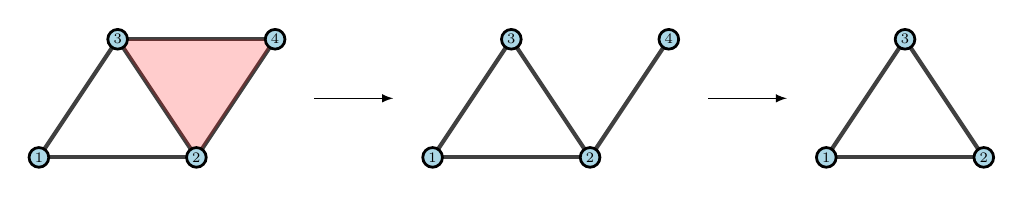
\begin{tikzpicture}
      \fill[opacity = 0.2, red] (2, 0) -- (1, 1.5) -- ( 3, 1.5) -- cycle; 
      \Vertex[x=0, y=0, size=0.25, fontscale=0.75, label=1]{v1}
      \Vertex[x=2, y=0, size=0.25, fontscale=0.75,label=2]{v2}
      \Vertex[x=1, y=1.5, size=0.25,fontscale=0.75, label=3]{v3}
      \Vertex[x=3, y=1.5, size=0.25,fontscale=0.75, label=4]{v4}
      \Edge(v1)(v2)
      \Edge(v1)(v3)
      \Edge(v2)(v3)
      \Edge(v2)(v4)
      \Edge(v3)(v4)

      \draw[-latex] ( 3.5, 0.75) -- (4.5, 0.75) ;

      \Vertex[x=5, y=0, size=0.25, fontscale=0.75, label=1]{v1}
      \Vertex[x=7, y=0, size=0.25, fontscale=0.75,label=2]{v2}
      \Vertex[x=6, y=1.5, size=0.25,fontscale=0.75, label=3]{v3}
      \Vertex[x=8, y=1.5, size=0.25,fontscale=0.75, label=4]{v4}
      \Edge(v1)(v2)
      \Edge(v1)(v3)
      \Edge(v2)(v3)
      \Edge(v2)(v4)

      \draw[-latex] ( 8.5, 0.75) -- (9.5, 0.75) ;

      \Vertex[x=10, y=0, size=0.25, fontscale=0.75, label=1]{v1}
      \Vertex[x=12, y=0, size=0.25, fontscale=0.75,label=2]{v2}
      \Vertex[x=11, y=1.5, size=0.25,fontscale=0.75, label=3]{v3}
      \Edge(v1)(v2)
      \Edge(v1)(v3)
      \Edge(v2)(v3)

\end{tikzpicture}}{Example of weakly collapsible but not collapsible simplicial complex \label{fig:weak_example}}
\end{example}

\begin{theorem}\label{thm:poly}
      Weak collapsibility of \( 2\)-skeleton \( \mc K \) is polynomially solvable.
\end{theorem}
\begin{proof}
      The \emph{greedy algorithm} for the collapsing sequence intuitively operates as follows: at each iteration perform any of possible collapses; in the absence of free edges, the complex should be considered not collapsible, \Cref{algo:greedy}. Clearly, such an algorithm runs polynomially with respect to the number of simplexes in \(\mc K\).
      % TODO:

      The failure of the greedy algorithm indicates the existence of a weakly collapsible complex \( \mc K \) such that the greedy algorithm gets stuck at a \( 2 \)-Core, which is avoidable for another possible order of collapses. Among all the counter exemplary complexes, let \( \mc K \) be a minimal one with respect to the number of triangles \( m_2 \). Then there exist a free edge \( \sigma \in \V 1 \) such that \( \mc K \backslash \{ \sigma \} \) is \emph{collapsible} and another \( \sigma' \in \V 2 \) such that \( \mc K \backslash \{ \sigma' \} \) is \emph{not collapsible}.

      Note that if \( \mc K \) is minimal then for any pair of free edges \( \sigma_1 \) and \( \sigma_2 \) belong to the same triangle: \( \tau(\sigma_1) = \tau(\sigma_2) \). Indeed, for any \( \tau(\sigma_1) \ne \tau(\sigma_2) \),  \( \mc K \backslash \{ \sigma_1, \sigma_2 \} = \mc K \backslash \{ \sigma_2, \sigma_1 \} \). Let \( \tau(\sigma_1) \ne \tau(\sigma_2) \) for at least one pair of \( \sigma_1 \) and \( \sigma_2 \); in our assumption, either both \( \mc K \backslash \{ \sigma_1 \} \) and \( \mc K \backslash \{ \sigma_2 \} \), only \( \mc K \backslash \{ \sigma_1 \}  \) or none are collapsible. In the former case either \( \mc K \backslash \{ \sigma_1 \} \) or \( \mc K \backslash \{ \sigma_2 \} \) is a smaller example of the complex satisfying the assumption, hence, violating the minimality. If only \( \mc K \backslash \{ \sigma_1 \} \) is collapsible, then \( \mc K \backslash \{ \sigma_2, \sigma_1 \}  \) is not collapsible; hence, \( \mc K \backslash \{ \sigma_1, \sigma_2 \} \) is not collapsible, so \( \mc K \backslash \{ \sigma_1 \} \) is a smaller example of a complex satisfying the assumption. Finally, if both \( \mc K \backslash \{ \sigma_1 \} \) and \( \mc K \backslash \{ \sigma_2 \} \) are collapsible, then for  known \( \sigma' \) such that \( \mc K \backslash \{ \sigma' \} \) is not collapsible, \( \tau(\sigma') \ne \tau(\sigma_1)\) or \( \tau(\sigma') \ne \tau(\sigma_2) \), which revisits the previous point.

      As a result, for \( \sigma \) ( \( \mc K \backslash \{ \sigma \} \) is collapsible) and for \( \sigma' \) ( \( \mc K \backslash \{ \sigma' \} \) is not collapsible ) it holds that \( \tau (\sigma) = \tau (\sigma') \Rightarrow  \sigma \cap \sigma' = \{ v \}  \), so after collapses \( \mc K  \{ \sigma \} \) and \( \mc K \backslash \{ \sigma' \} \) we arrive at two identical simplicial complexes modulo the hanging vertex irrelevant for the weak collapsibility. A simplicial complex can not be simultaneously collapsible and not collapsible, so the question of weak collapsibility can always be resolved by the greedy algorithm which has polynomial complexity.
\end{proof}

\begin{comment}
\blav
\begin{remark}
      The proof above is reminiscent of the one for polynomiality of \(d\)-collapsibility, \( d = 1\) or \( d = 2\), \cite{tancer2008dcollapse}, but bares significant differences: firstly, \( 2 \)-collapsibility allows collapses at \(\sigma: \; \dim \sigma \le 1\); secondly, in the scope of \cite{tancer2008dcollapse}, \( \tau(\sigma) = \sigma \) is allowed which affects (complicates) the proof.
\end{remark}
\elav


\begin{remark}
      If \( \mc K \) is weakly collapsible, then the number of triangles can not be higher than the number of edges, \( m_2 \le m_1 \), hence \( \mc K \) is \emph{necessarily sparse} and does not breach the gap up to \( m_2 = \mc O\left( m_1 \ln \left( 4 m_1 \right) \right) \).
\end{remark}
\end{comment}

\subsection{Computational cost of the greedy algorithm}

Let \( \mc K \) be a \(2\)-skeleton; let \( \Delta_\sigma \) be a set of triangles of \( \mc K \) containing the edge \( \sigma \), \( \Delta_\sigma = \{ t \mid  t \in \V 2  \text{ and } \sigma \in t \} \). Then the edge \( \sigma \) is free iff \( | \Delta_\sigma | = 1 \) and \( F = \{ \sigma \mid | \Delta_e | = 1  \} \) is a set of all free edges. Note that \( | \Delta_e | \le m_0 -2 = \mc O ( m_0  ) \).

\begin{algorithm}[h]
      \caption{ \texttt{GREEDY\_COLLAPSE}(\(\mc K\)):  greedy algorithm for the weak collapsibility
      \label{algo:greedy}}
      \begin{algorithmic}[1]
            \Require initial set of free edges \( F \), adjacency sets \(  \{ \Delta_{ \sigma_i } \}_{i=1}^{ m_1 } \)
             \State \( \Sigma = [ \; ] , \; \ds T = [ \; ] \) \Comment{ initialize the collapsing sequence}
             \While{ \( F \ne \vn \) \textbf{ and } \( \V 2 \ne \vn \) }
                  \State \( \sigma \gets \texttt{pop}( F ) \), \( \; \tau \gets \tau(\sigma)  \) \Comment{ pick a free edge \( \sigma \) }
                  \State \( \mc K \gets \mc K \backslash \{ \sigma \} \), \( \; \Sigma \gets [ \, \Sigma \;\; \sigma \, ] , \; \ds T \gets [ \ds T \; \tau ] \) \Comment{ \small \( \tau \) is a triangle being collapsed; \( \tau = [ \sigma, \sigma_1, \sigma_2 ] \) }
                  \State \( \Delta_{\sigma_1} \gets \Delta_{\sigma_1} \backslash \tau  \), \( \; \Delta_{\sigma_2} \gets \Delta_{\sigma_2} \backslash \tau  \) \Comment{ remove \( \tau \) from adjacency lists }
                  \State \( F \gets F \cup \{ \sigma_i \, |  \, i = 1, 2 \text{ and } | \Delta_{\sigma_i} | = 1 \}  \) \Comment{ update \( F \) if any of \( \sigma_1 \) or \( \sigma_2 \) has become free }
                  %\State \( \mc K \gets \mc K  \backslash \{ \sigma \} \) \Comment{ perform a collapse  }
             \EndWhile
             \State \Return \( \mc K, \, \Sigma, \, \ds T \)
      \end{algorithmic}
\end{algorithm}

The complexity of \Cref{algo:greedy} rests upon the precomputed \( \sigma \mapsto \Delta_\sigma \) structure that de-facto coincides with the boundary operator \( B_2 \) (assuming \( B_2 \) is stored as a sparse matrix, the adjacency structure describes its non-zero entries). Similarly, the initial \( F \) set can be computed alongside the construction of \( B_2 \) matrix. Another concession is needed for the complexity of the removal of elements from \( \Delta_{\sigma_i} \) and \( F \), which may vary from \( \mc O (1) \) on average up to guaranteed \( \log ( | \Delta_{\sigma_i} | ) \). As a result, given a pre-existing \( B_2 \) operator, \Cref{algo:greedy} runs linearly, \( \mc O ( m_1  )\), or almost linearly depending on the realisation, \( \mc O ( m_1 \log m_1 )\).











%----------------------------------------------------------------------------------------
%	THESIS CONTENT - APPENDICES
%----------------------------------------------------------------------------------------

\addtocontents{toc}{\vspace{2em}} % Add a gap in the Contents, for aesthetics
%
\appendix % Cue to tell LaTeX that the following 'chapters' are Appendices

%% Include the appendices of the thesis as separate files from the Appendices folder
%% Uncomment the lines as you write the Appendices

%%----------------------------------------------------------------------------------------
%	Appendix A
%----------------------------------------------------------------------------------------
\chapter{Appendix Title Here}\label{app:appendixA}

\todo{Write your Appendix content here, if needed.}
%\input{./Appendices/AppendixB}
%\input{./Appendices/AppendixC}

%\addtocontents{toc}{\vspace{2em}} % Add a gap in the Contents, for aesthetics
%
%\backmatter

\clearpage

%----------------------------------------------------------------------------------------
%	BIBLIOGRAPHY
%----------------------------------------------------------------------------------------

\nocite{*}

\label{Bibliography}

\lhead{\emph{Bibliography}} % Change the page header to say "Bibliography"

\bibliographystyle{unsrtnat} % Use the "unsrtnat" BibTeX style for formatting the Bibliography

\bibliography{notes} % The references (bibliography) information are stored in the file named "Bibliography.bib"

\end{document}